% !TeX program  = xelatex
% !TeX encoding = UTF-8
% !TeX root     = course-work.tex
\documentclass{mirea}

% !TeX program  = xelatex
% !TeX encoding = UTF-8
% !TeX root     = article1.tex

\usepackage{hyperref}
\hypersetup{pdftitle={ВКР на тему "<Разработка системы для поиска и возврата утерянных вещей">}, pdfauthor={В. С. Верхотуров}}

\usepackage{comment}

\usepackage{graphicx}

\usepackage{listings}
\usepackage{xcolor}
\lstset{basicstyle=\footnotesize, breaklines=true, numbers=left, captionpos=t, showstringspaces=false, commentstyle=\color{teal}, stringstyle=\color{red}, keywordstyle=\color{violet}}  % Настройки, применяемые ко всем листингам

% Создание введения или заключения
\newcommand{\supersection}[1]{
	\section*{#1}
	\phantomsection
	\addcontentsline{toc}{section}{#1}
}

\usepackage{caption}
\captionsetup[lstlisting]{justification=raggedright, singlelinecheck=false}

\usepackage{pdfpages}

\usepackage{microtype}

\usepackage{multirow}

\usepackage{array}
\usepackage{setspace}
\newcolumntype{x}[1]{>{\setstretch{0.8}\small\centering\arraybackslash\hspace{0pt}}m{#1}}
\newcolumntype{y}[1]{>{\centering\arraybackslash\hspace{0pt}}m{#1}}
\usepackage{longtable}

\usepackage{float}

%\usepackage{color,xesearch}
%\SearchList{make-red}{\textcolor{red}{#1}}{эффективность,эффективности,эффективностью,эффективностей,эффективностям,эффективностями,эффективностях,эффективный,эффективная,эффективное,инновационный,иновационная,иновационные,инновация,иновационных,надежность,оптимизация,качество}


\begin{document}
	
% 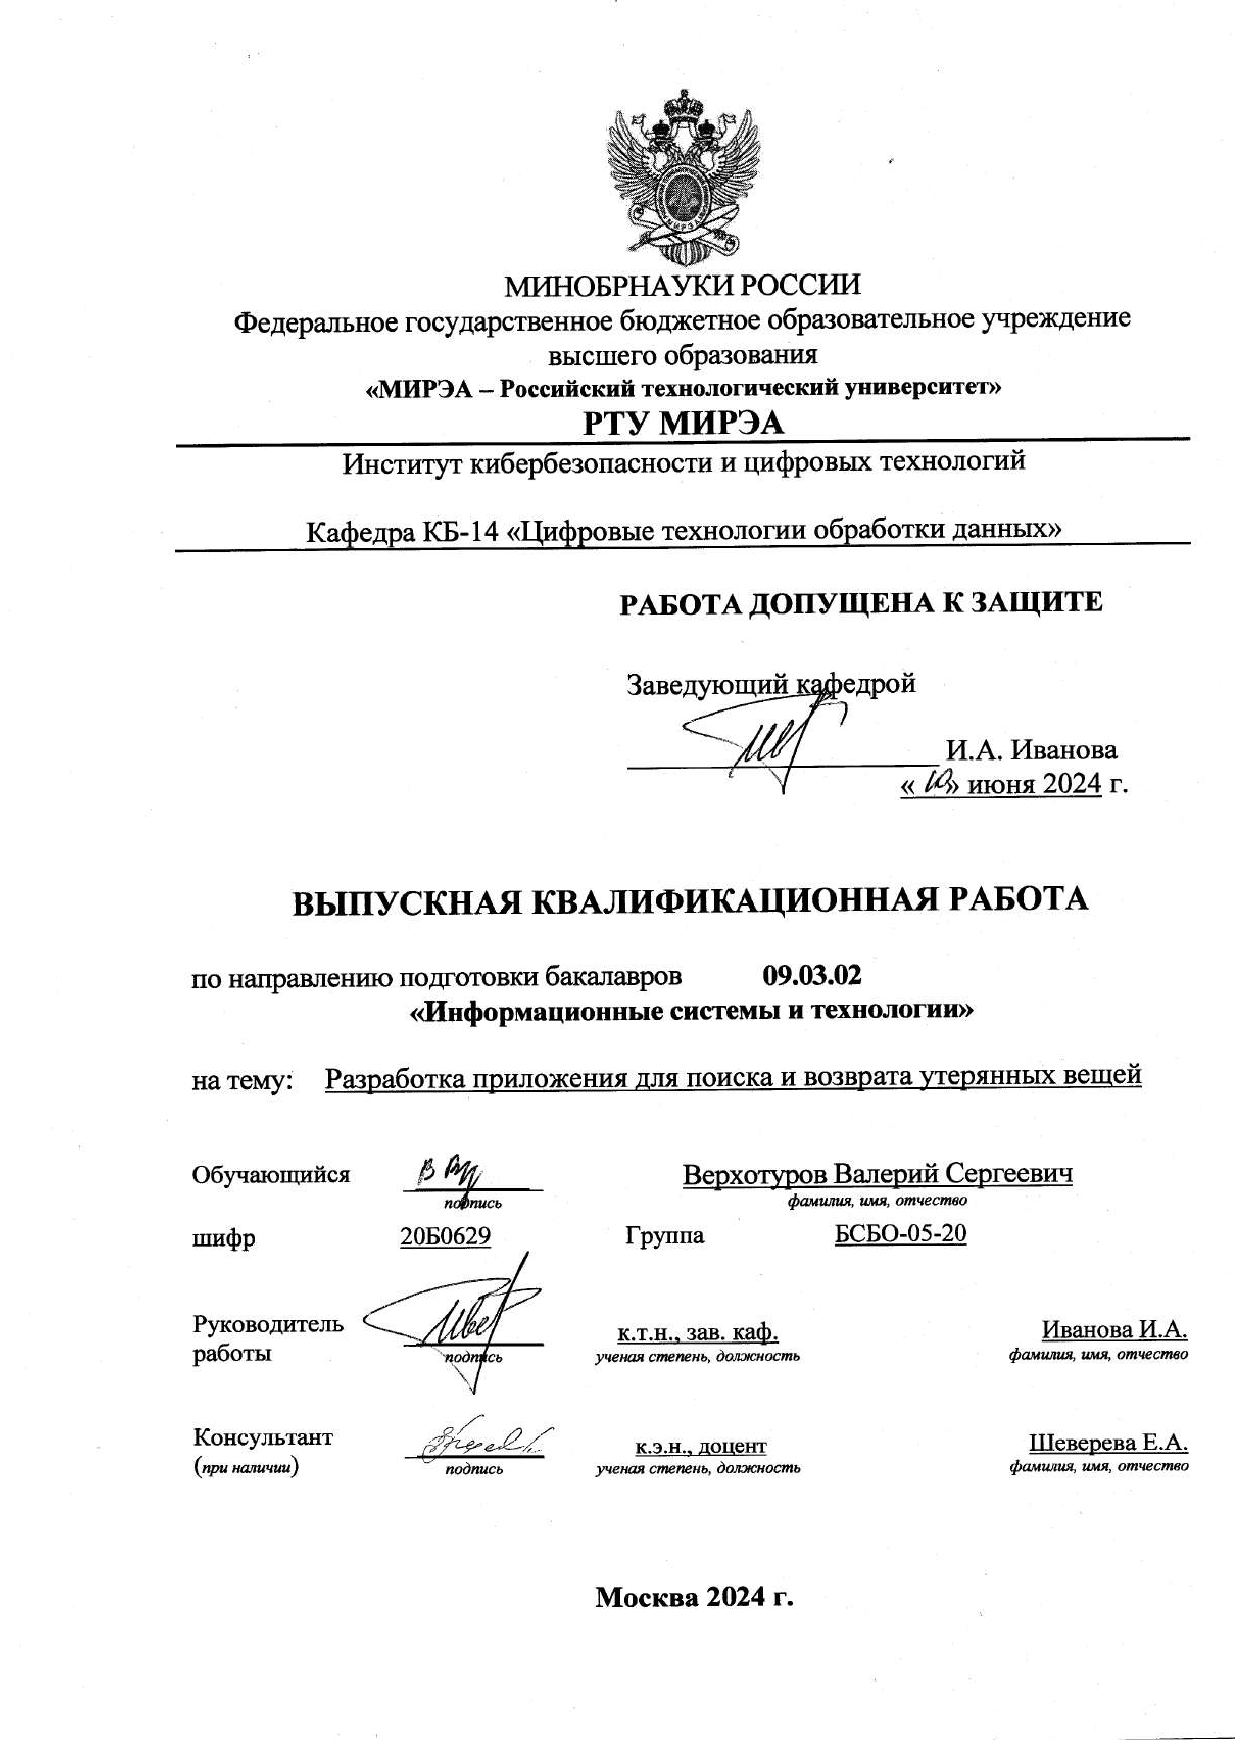
\includepdf[pages=-]{titlepage.pdf}

\begin{comment}
\begin{titlepage}
	\pagestyle{empty}
	\setlength\parindent{0pt}
	\newcommand{\blankDate}[2]{\mbox{\uline{<<\makebox[.7cm]{#1}>>~\makebox[2cm]{#2}~\the\year{}~г.}}} % {день}{месяц}
	\newcommand\blankLine[2]{$\underset{\text{#1}}{\text{\uline{#2}}}$}
	\begin{center}
		\includegraphics[width=2.5cm]{images/MIREA_Gerb_Black} \par
		МИНОБРНАУКИ РОССИИ \par 
		Федеральное государственное бюджетное образовательное учреждение высшего образования \par
		\textbf{<<МИРЭА~--- Российский технологический университет>>} \par
		\textbf{\fontsize{16pt}{16pt}\selectfont РТУ МИРЭА} \par
		\blankLine{(наименование института, филиала)}{Институт кибербезопасности и цифровых технологий} \par
		\blankLine{(наименование кафедры)}{Кафедра КБ-14 <<Цифровые технологии обработки данных>>} 
		\vspace*{.5cm}\par
		{\fontsize{16pt}{16pt}\selectfont
			\textbf{ОТЧЕТ ПО ПРОИЗВОДСТВЕННОЙ ПРАКТИКЕ}} \par
		\textbf{<<Технологическая (проектно-ориентированная) практика>>}
	\end{center}
	\textbf{Тема практики \uline{Разработка приложения для поиска и возврата утерянных вещей}} \bigskip\par
	Студент группы \blankLine{учебная группа, фамилия, имя, отчество студента}{БСБО-05-20 В.~С.~Верхотуров\hspace{3cm}} \hfill\blankLine{подпись студента}{\hspace{3cm}} \bigskip\par
	Руководитель курсовой работы \blankLine{должность, звание, учёная степень}{\hspace{6cm}} \hfill\blankLine{подпись руководителя}{\hspace{3cm}} \bigskip\par
	Рецензент (при наличии) \blankLine{должность, звание, учёная степень}{\hspace{7cm}} \hfill\blankLine{подпись рецензента}{\hspace{3cm}} \bigskip\par
	\begin{tabular}{@{}ll}
		Работа предоставлена к защите & \blankDate{}{} \bigskip\\
		Допущен к защите & \blankDate{}{}
	\end{tabular}
	\begin{center}
		\vfill Москва~--- \the\year{}~г.
	\end{center}
\end{titlepage}
\end{comment}
	
\addtocounter{page}{2}

% Содержание
\tableofcontents

% Введение
\supersection{Введение}
\label{sec:introduction}

Поиск утерянных вещей является актуальной проблемой, которая возникает при различных обстоятельствах. Эта проблема может возникнуть в результате потери ключей, документов, мобильных телефонов, кошельков или других ценных или важных вещей. В связи с этим существует необходимость разработки системы, которая поможет людям вернуть утерянные вещи.

Целью данной работы является разработка системы для поиска утерянных вещей на основе анализа существующих систем и технологий, а также определение требований к системе и ее функциональности. Для достижения этой цели будут рассмотрены различные методы и технологии, которые могут быть использованы для создания такой системы.

В разделе~\ref{sec:analytics} будет проведен анализ существующих систем поиска утерянных вещей и выделены их преимущества и недостатки. В разделе~\ref{sec:special} будут определены требования к разрабатываемой системе, рассмотрены методы и технологии, которые можно использовать для реализации системы. Раздел~\ref{sec:technology} будет посвящена описанию процесса разработки и тестирования системы. В разделе~\ref{sec:economy} будет приведен план разработки и расчет сметы затрат.

Таким образом, разработка системы для поиска утерянных вещей позволит создать удобный инструмент для поиска потерянных вещей, что приведет к уменьшению количества потерянных вещей и улучшению качества жизни людей.

% Аналитический раздел
\section{Аналитический раздел}
\label{sec:analytics}

\subsection{Статистика потерянных и найденных вещей}

Для подтверждения актуальности и важности разрабатываемой системы, необходимо провести исследование рынка и определить основные проблемы и потребности пользователей. Одним из способов сбора информации является проведение опроса среди пользователей.

Одним из основных факторов, определяющих актуальность разрабатываемой системы является статистика потерянных и найденных вещей. Необходимо определить количество потерянных вещей в месяц, год и за весь период работы системы. Это поможет оценить нагрузку на систему и определить ее производительность.

Статистика, взятая с сайта столнаходок.рф~\cite{bib:stol_nahodok}, утверждает, что только 20~\% пользователей их сайта смогли установить и вернуть вещи. Также на рисунках \ref{fig:chart2023} и \ref{fig:chart2022} представлена гистограмма количества созданных объявлений за 2022 и 2023 года.

\begin{figure}[htb]
	\centering
	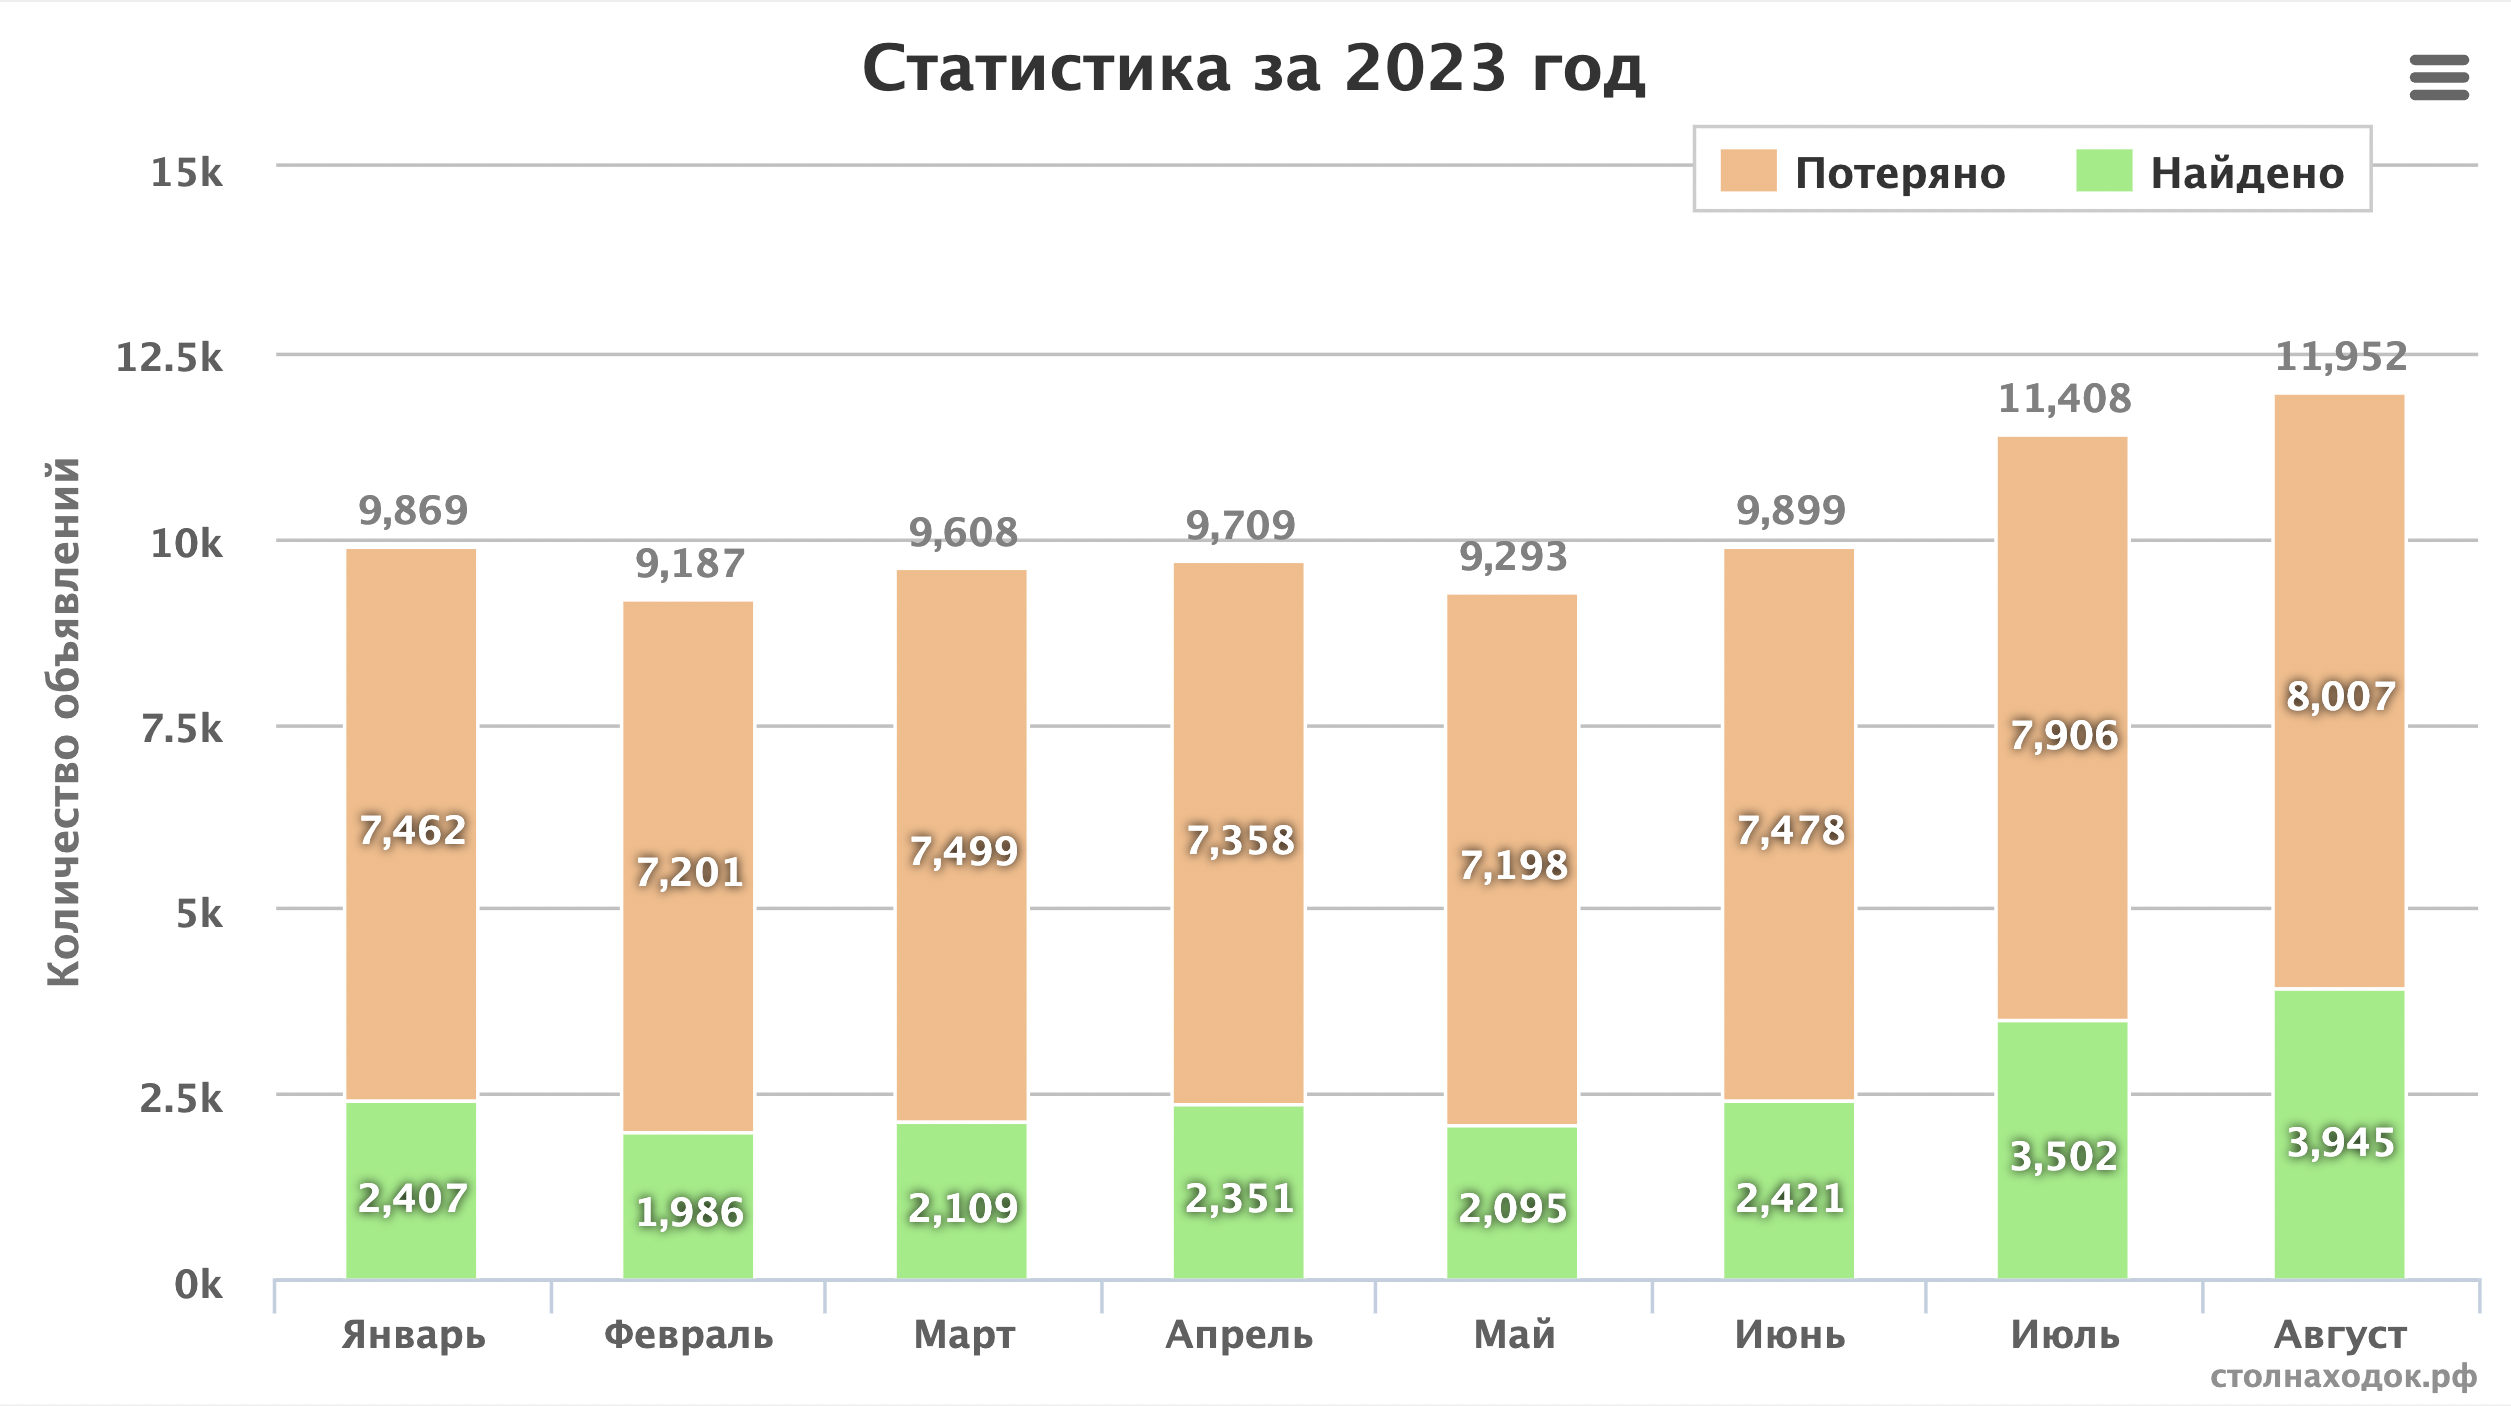
\includegraphics[width=.6\textwidth]{images/chart2023}
	\parskip=6pt
	\caption{Востребованность системы столнаходок.рф в 2023 году}
	\label{fig:chart2023}
\end{figure}

\begin{figure}[htb]
	\centering
	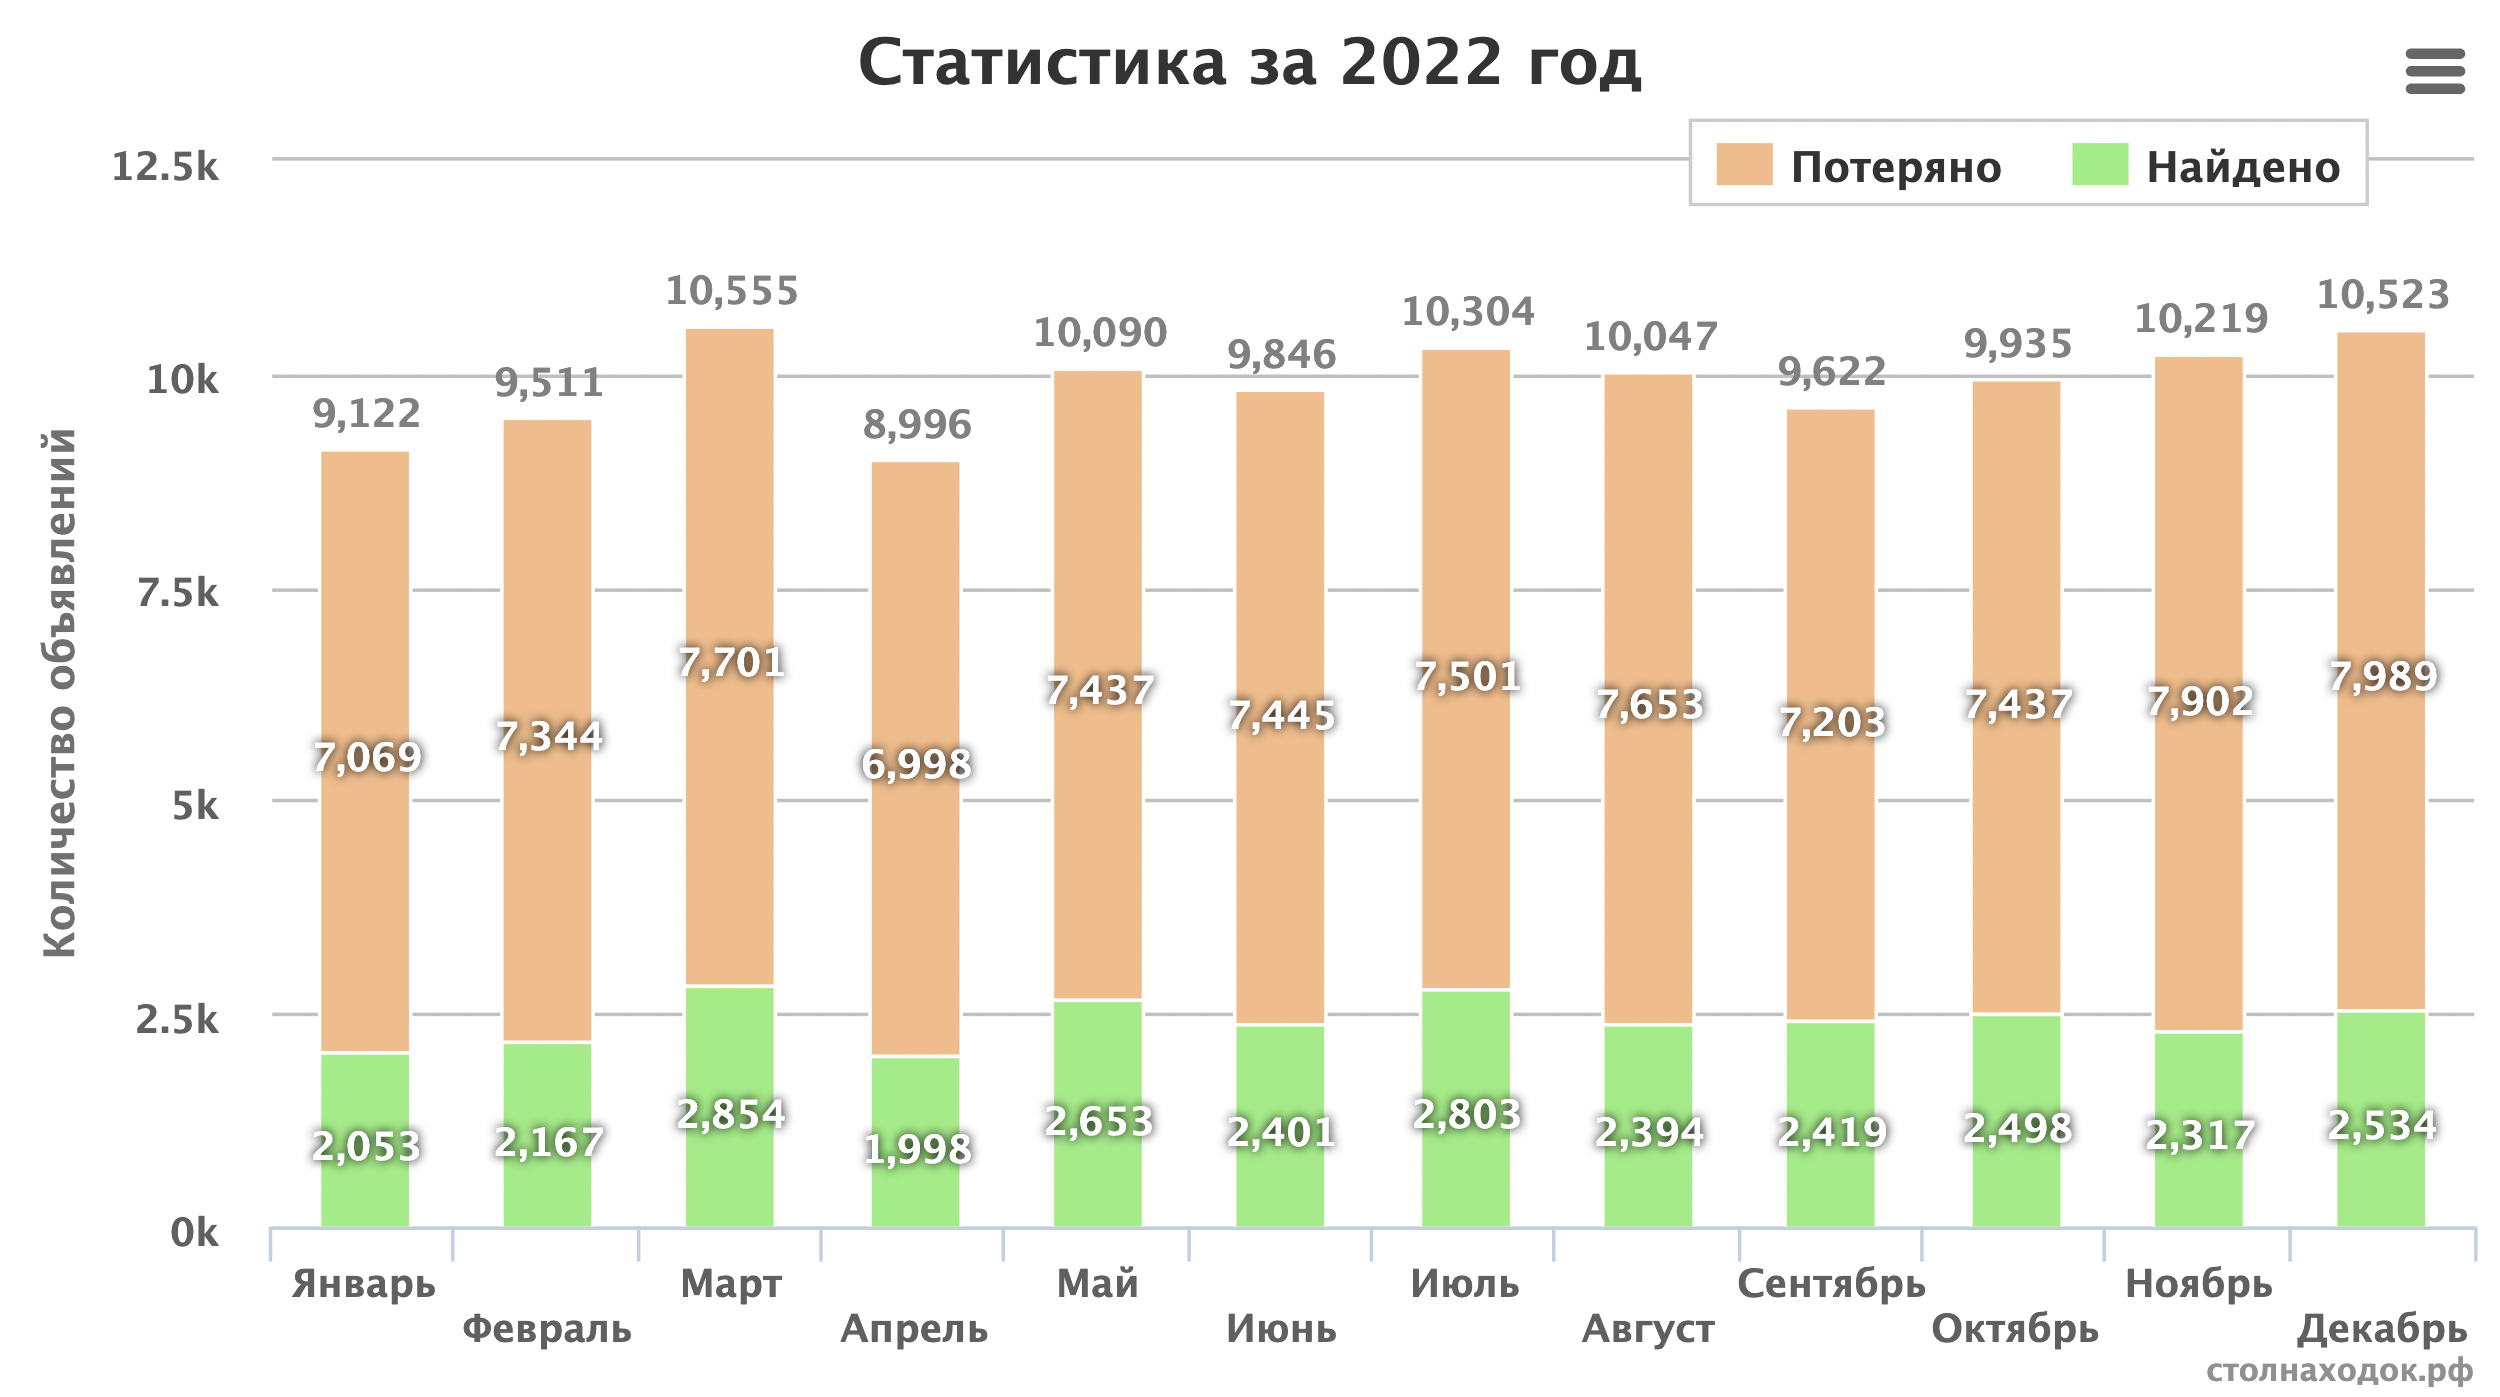
\includegraphics[width=.6\textwidth]{images/chart2022}
	\parskip=6pt
	\caption{Востребованность системы столнаходок.рф в 2022 году}
	\label{fig:chart2022}
\end{figure}

\subsection{Типы существующих решений для поиска и возврата утерянных вещей}

Существует несколько типов существующих решений для поиска и возврата утерянных вещей. Ниже приведены некоторые из них:
\begin{enumerate}
	\item Веб-сайты и мобильные приложения: <<Бюро находок>>~\cite{bib:stol_nahodok,bib:pona}. Эти сервисы предоставляют платформу, где люди могут регистрировать утерянные вещи и искать их владельцев. Пользователям предлагается создать объявления о найденных или потерянных вещах и связаться друг с другом, чтобы вернуть вещи. Некоторые сервисы предлагают добавить фотографии или описание вещей, чтобы облегчить поиск. 
	
	\item Технология RFID (Radio Frequency Identification) позволяет прикреплять RFID-метки к ценным объектам и определить владельца с помощью специальных считывателей~\cite{bib:investopedia_rfid,bib:airtag}. Это возможно благодаря использованию радиоволн, которые позволяют быстро определять местоположение потерянных вещей с помощью дополнительного программного обеспечения. Одним из наиболее распространенных применений технологии RFID является микрочипирование домашних животных или чипов для домашних животных. Эти микрочипы имплантируются ветеринарами и содержат информацию, касающуюся домашних животных, включая их имя, медицинские записи и контактную информацию их владельцев. Если домашнее животное пропадает и его отправляют в спасательную службу или в приют, работник приюта сканирует животное на наличие микрочипа. Если у домашнего животного есть микрочип, работнику приюта достаточно одного телефонного звонка или поиска в Интернете, чтобы связаться с владельцами домашнего животного. Считается, что чипы для домашних животных более надежны, чем ошейники, которые можно упасть или снять.
	
	\item GPS-трекеры --- это устройства с встроенным GPS-модулем. Они могут быть прикреплены практически к любому объекту, после чего его местоположение определяется через смартфон или компьютер по сети Интернет. При использовании приложения на смартфоне пользователь может получать уведомления о передвижении объекта и быстро определять его текущее местоположение.
	
	\item Автоматизированные системы поиска утерянных предметов: Некоторые организации, например, аэропорты и железнодорожные станции, используют системы обнаружения утерянных предметов. В этих системах используются технологии, такие как видеонаблюдение, детекторы движения и распознавание образов для отслеживания и возвращения потерянных предметов их владельцам.
\end{enumerate}

Каждый из этих типов решений имеет свои преимущества и недостатки. Некоторые из них могут быть более подходящими для конкретных ситуаций, например, GPS-трекеры могут быть полезными при поиске утерянных вещей на открытой местности, в то время как RFID-метки могут быть более подходящими для использования внутри помещений. Веб-сайты и приложения <<Бюро находок>> предоставляют более универсальное решение, которое может быть использовано в различных ситуациях.

\subsection{Анализ существующих систем для поиска и возврата утерянных вещей}

В настоящем разделе будет проведен обзор существующих сервисов и приложений, которые предлагают функциональность поиска и возврата утерянных вещей. Данный обзор позволит выявить основные преимущества и недостатки этих сервисов, а также определить потенциальные возможности для улучшения их функциональности.

<<столнаходок.рф>>~\cite{bib:stol_nahodok} --- это один из наиболее популярных веб-сервисов, предоставляющих возможность объявлять о потерянных и найденных предметах. Сервис имеет простой и интуитивно понятный интерфейс, позволяющий пользователям быстро разместить информацию о потерянных вещах и связаться с владельцами найденных предметов, примеры пользовательского интерфейса представлены на рис.~\ref{fig:stolNahodok1}, \ref{fig:stolNahodok2}. Однако, отсутствие системы уведомлений и неудобное сопоставление объявлений ограничивают его функциональность.

\begin{figure}[htb]
	\centering
	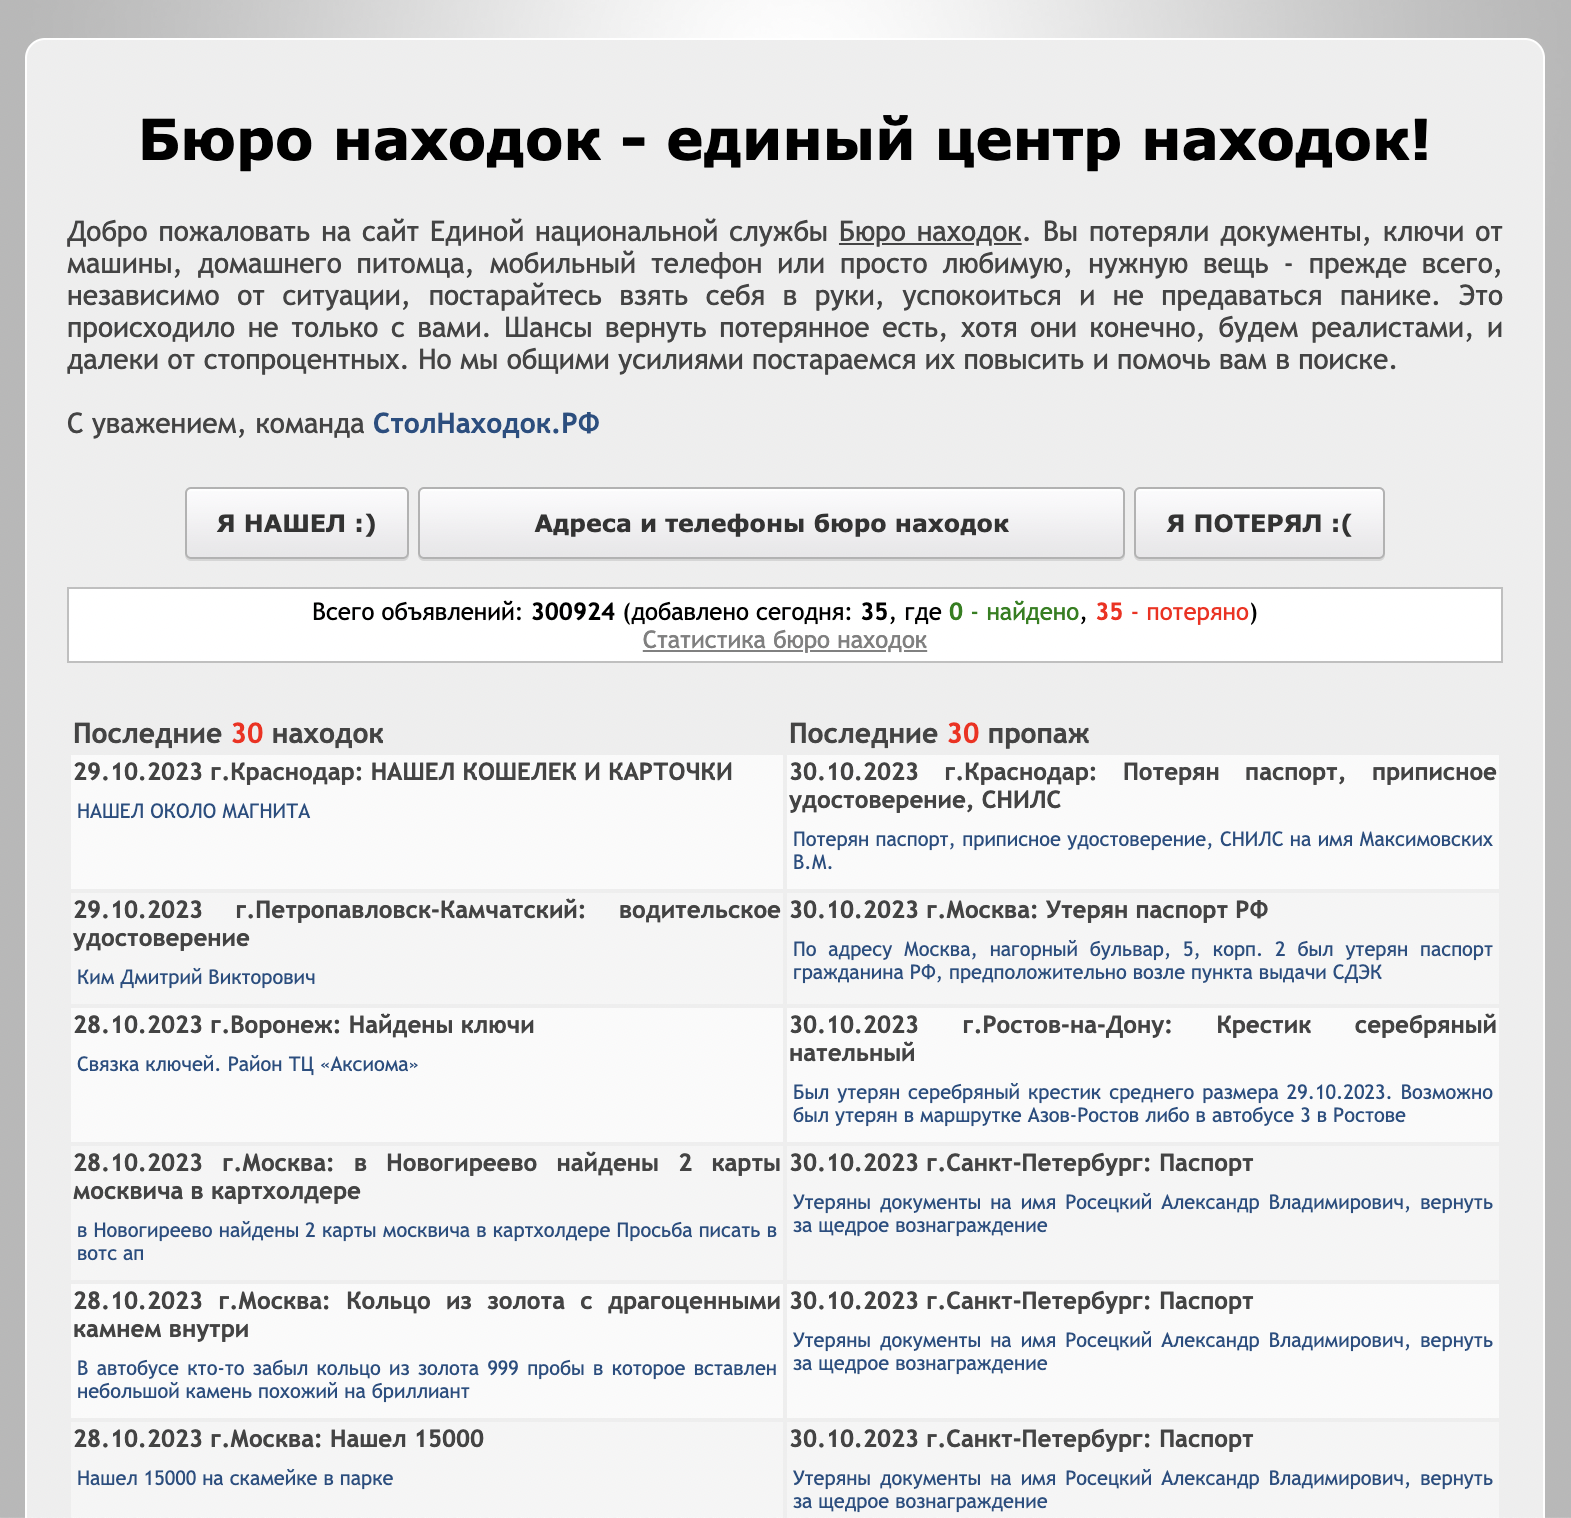
\includegraphics[width=.95\textwidth]{images/stolNahodok1}
	\parskip=6pt
	\caption{Скриншот системы <<столнаходок.рф>>}
	\label{fig:stolNahodok1}
\end{figure}

\begin{figure}[htb]
	\centering
	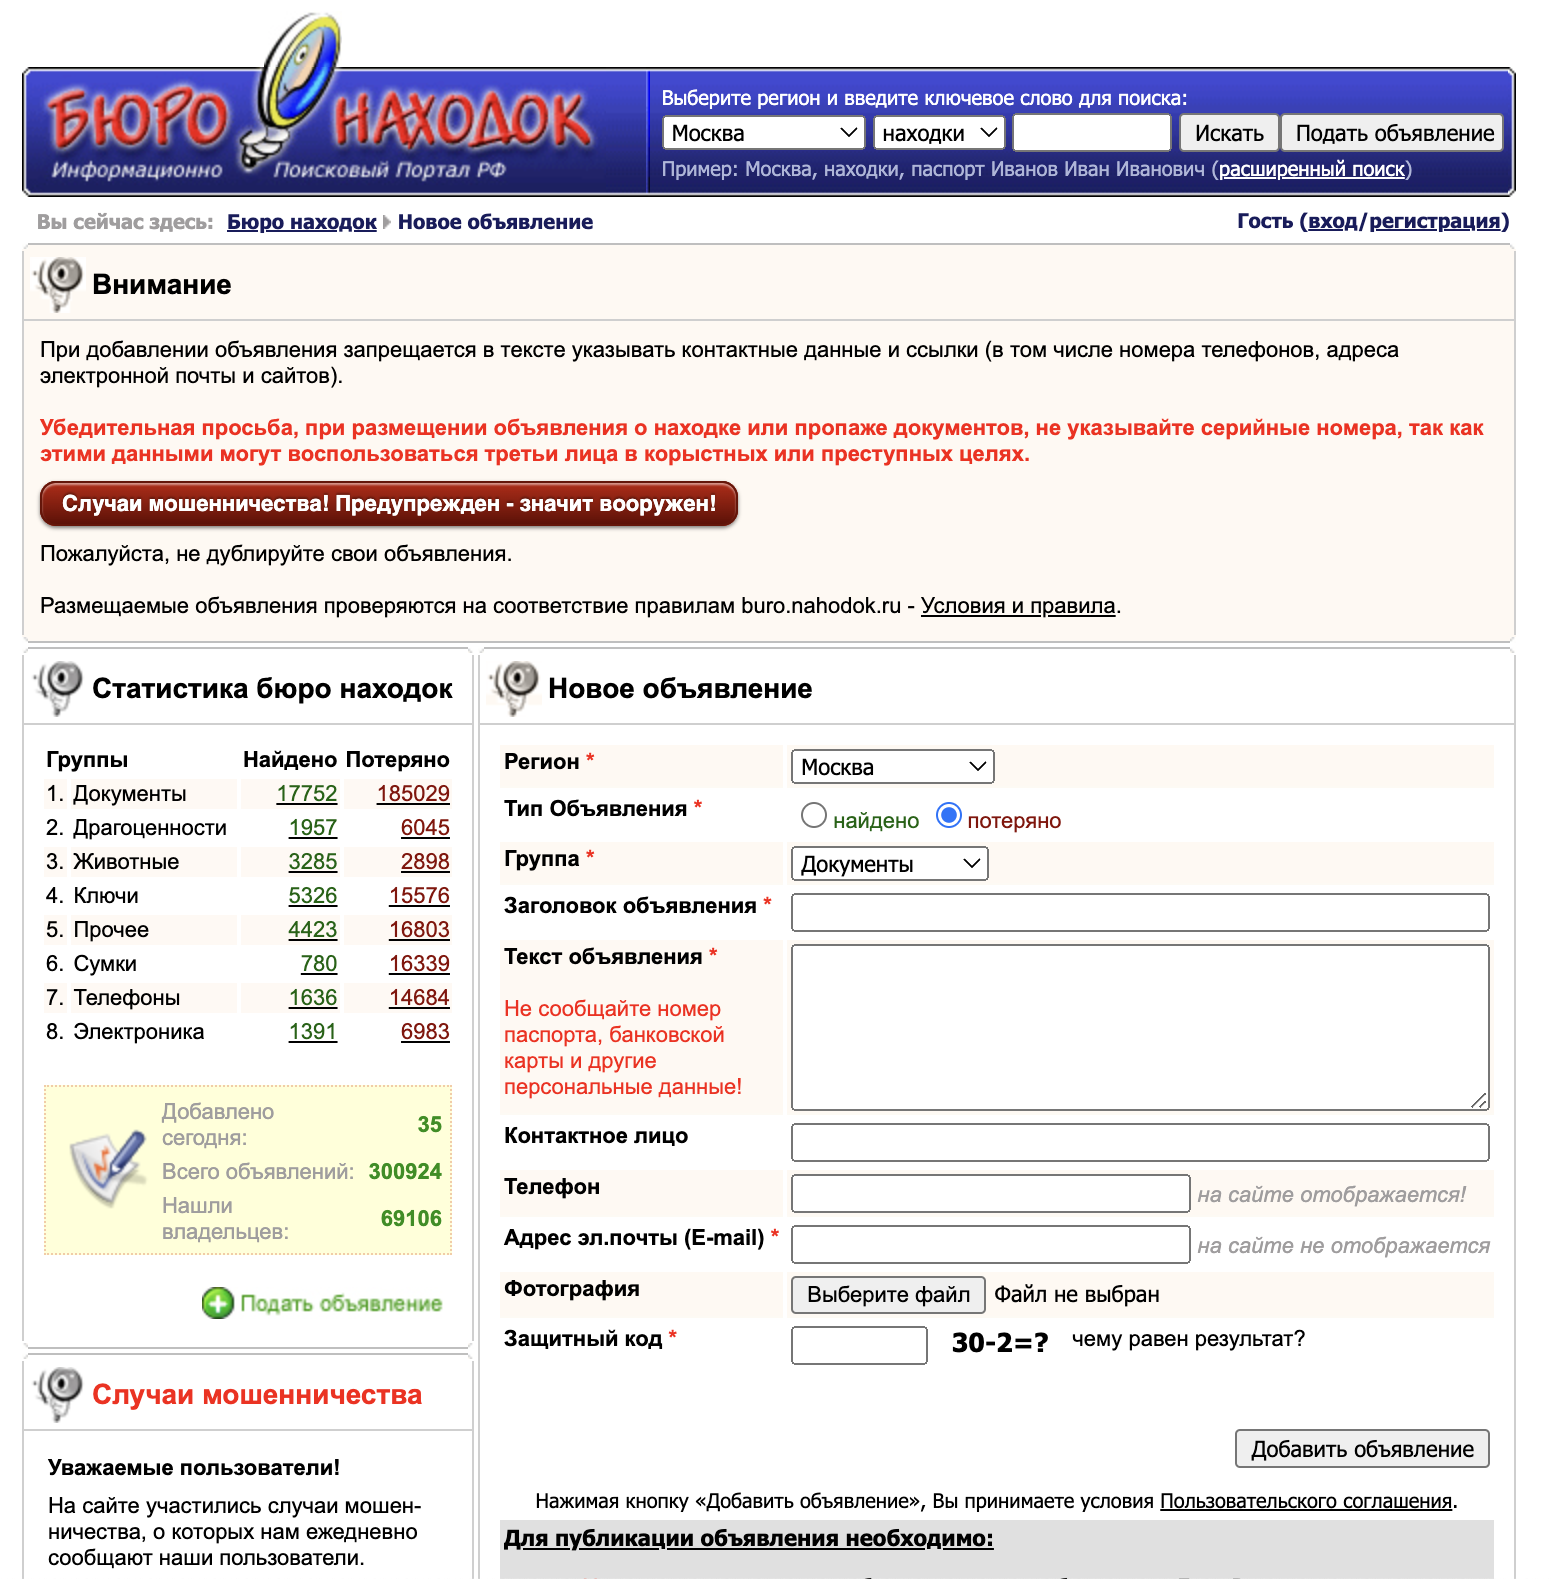
\includegraphics[width=.95\textwidth]{images/stolNahodok2}
	\parskip=6pt
	\caption{Скриншот системы <<столнаходок.рф>>}
	\label{fig:stolNahodok2}
\end{figure}

<<Find My Stuff>>~\cite{bib:find_my_stuff} --- это мобильное приложение, разработанное для операционных систем iOS и Android. Оно предлагает функцию отслеживания утерянных предметов через GPS-модуль смартфона, представлено на рис.~\ref{fig:findMyStuff1}, \ref{fig:findMyStuff2}. Пользователи могут отмечать свои вещи на карте и получать уведомления, когда они находятся рядом с утерянным предметом. Однако, ограничение использования только наличием смартфона с GPS-модулем и низкая точность определения местоположения представляют существенные ограничения данного приложения.

\begin{figure}[htb]
	\centering
	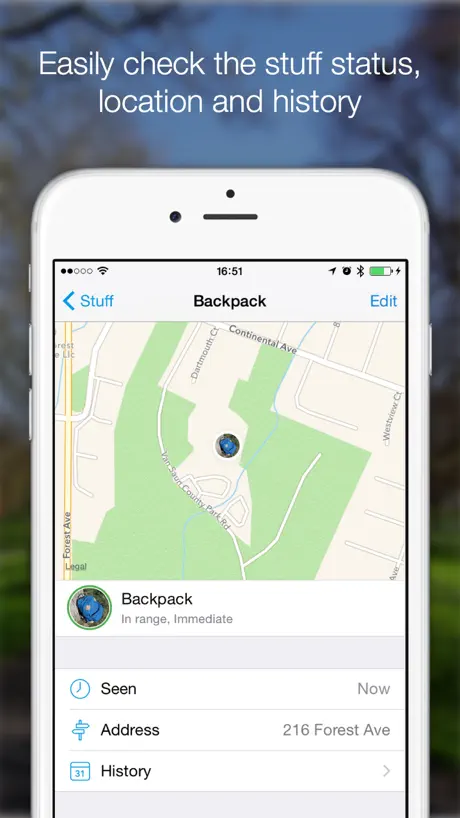
\includegraphics[height=.4\textheight]{images/findMyStuff1.png}
	\parskip=6pt
	\caption{Скриншот системы <<Find My Stuff>>}
	\label{fig:findMyStuff1}
\end{figure}

\begin{figure}[htb]
	\centering
	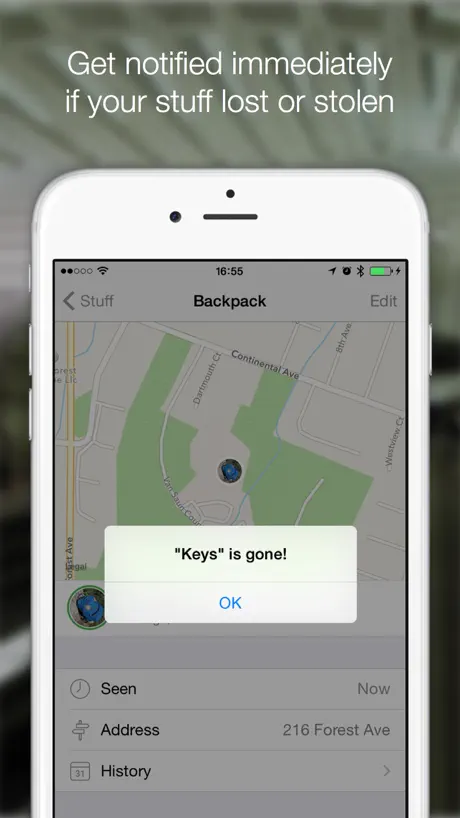
\includegraphics[height=.4\textheight]{images/findMyStuff2.png}
	\parskip=6pt
	\caption{Скриншот системы <<Find My Stuff>>}
	\label{fig:findMyStuff2}
\end{figure}

<<Lost Property Office>>~\cite{bib:parliament_lost_and_found} --- это веб-сервис, предоставляемый государственными организациями и органами правопорядка, см. рис.~\ref{fig:lostPropertyOffice}. Сервис позволяет пользователям сообщать о потерянных и найденных предметах, а также предоставляет информацию о процедуре возврата утерянных вещей. Однако, ограниченный доступ к сервису и неудобный процесс регистрации и подачи заявки являются значительными недостатками данного сервиса.

\begin{figure}[htb]
	\centering
	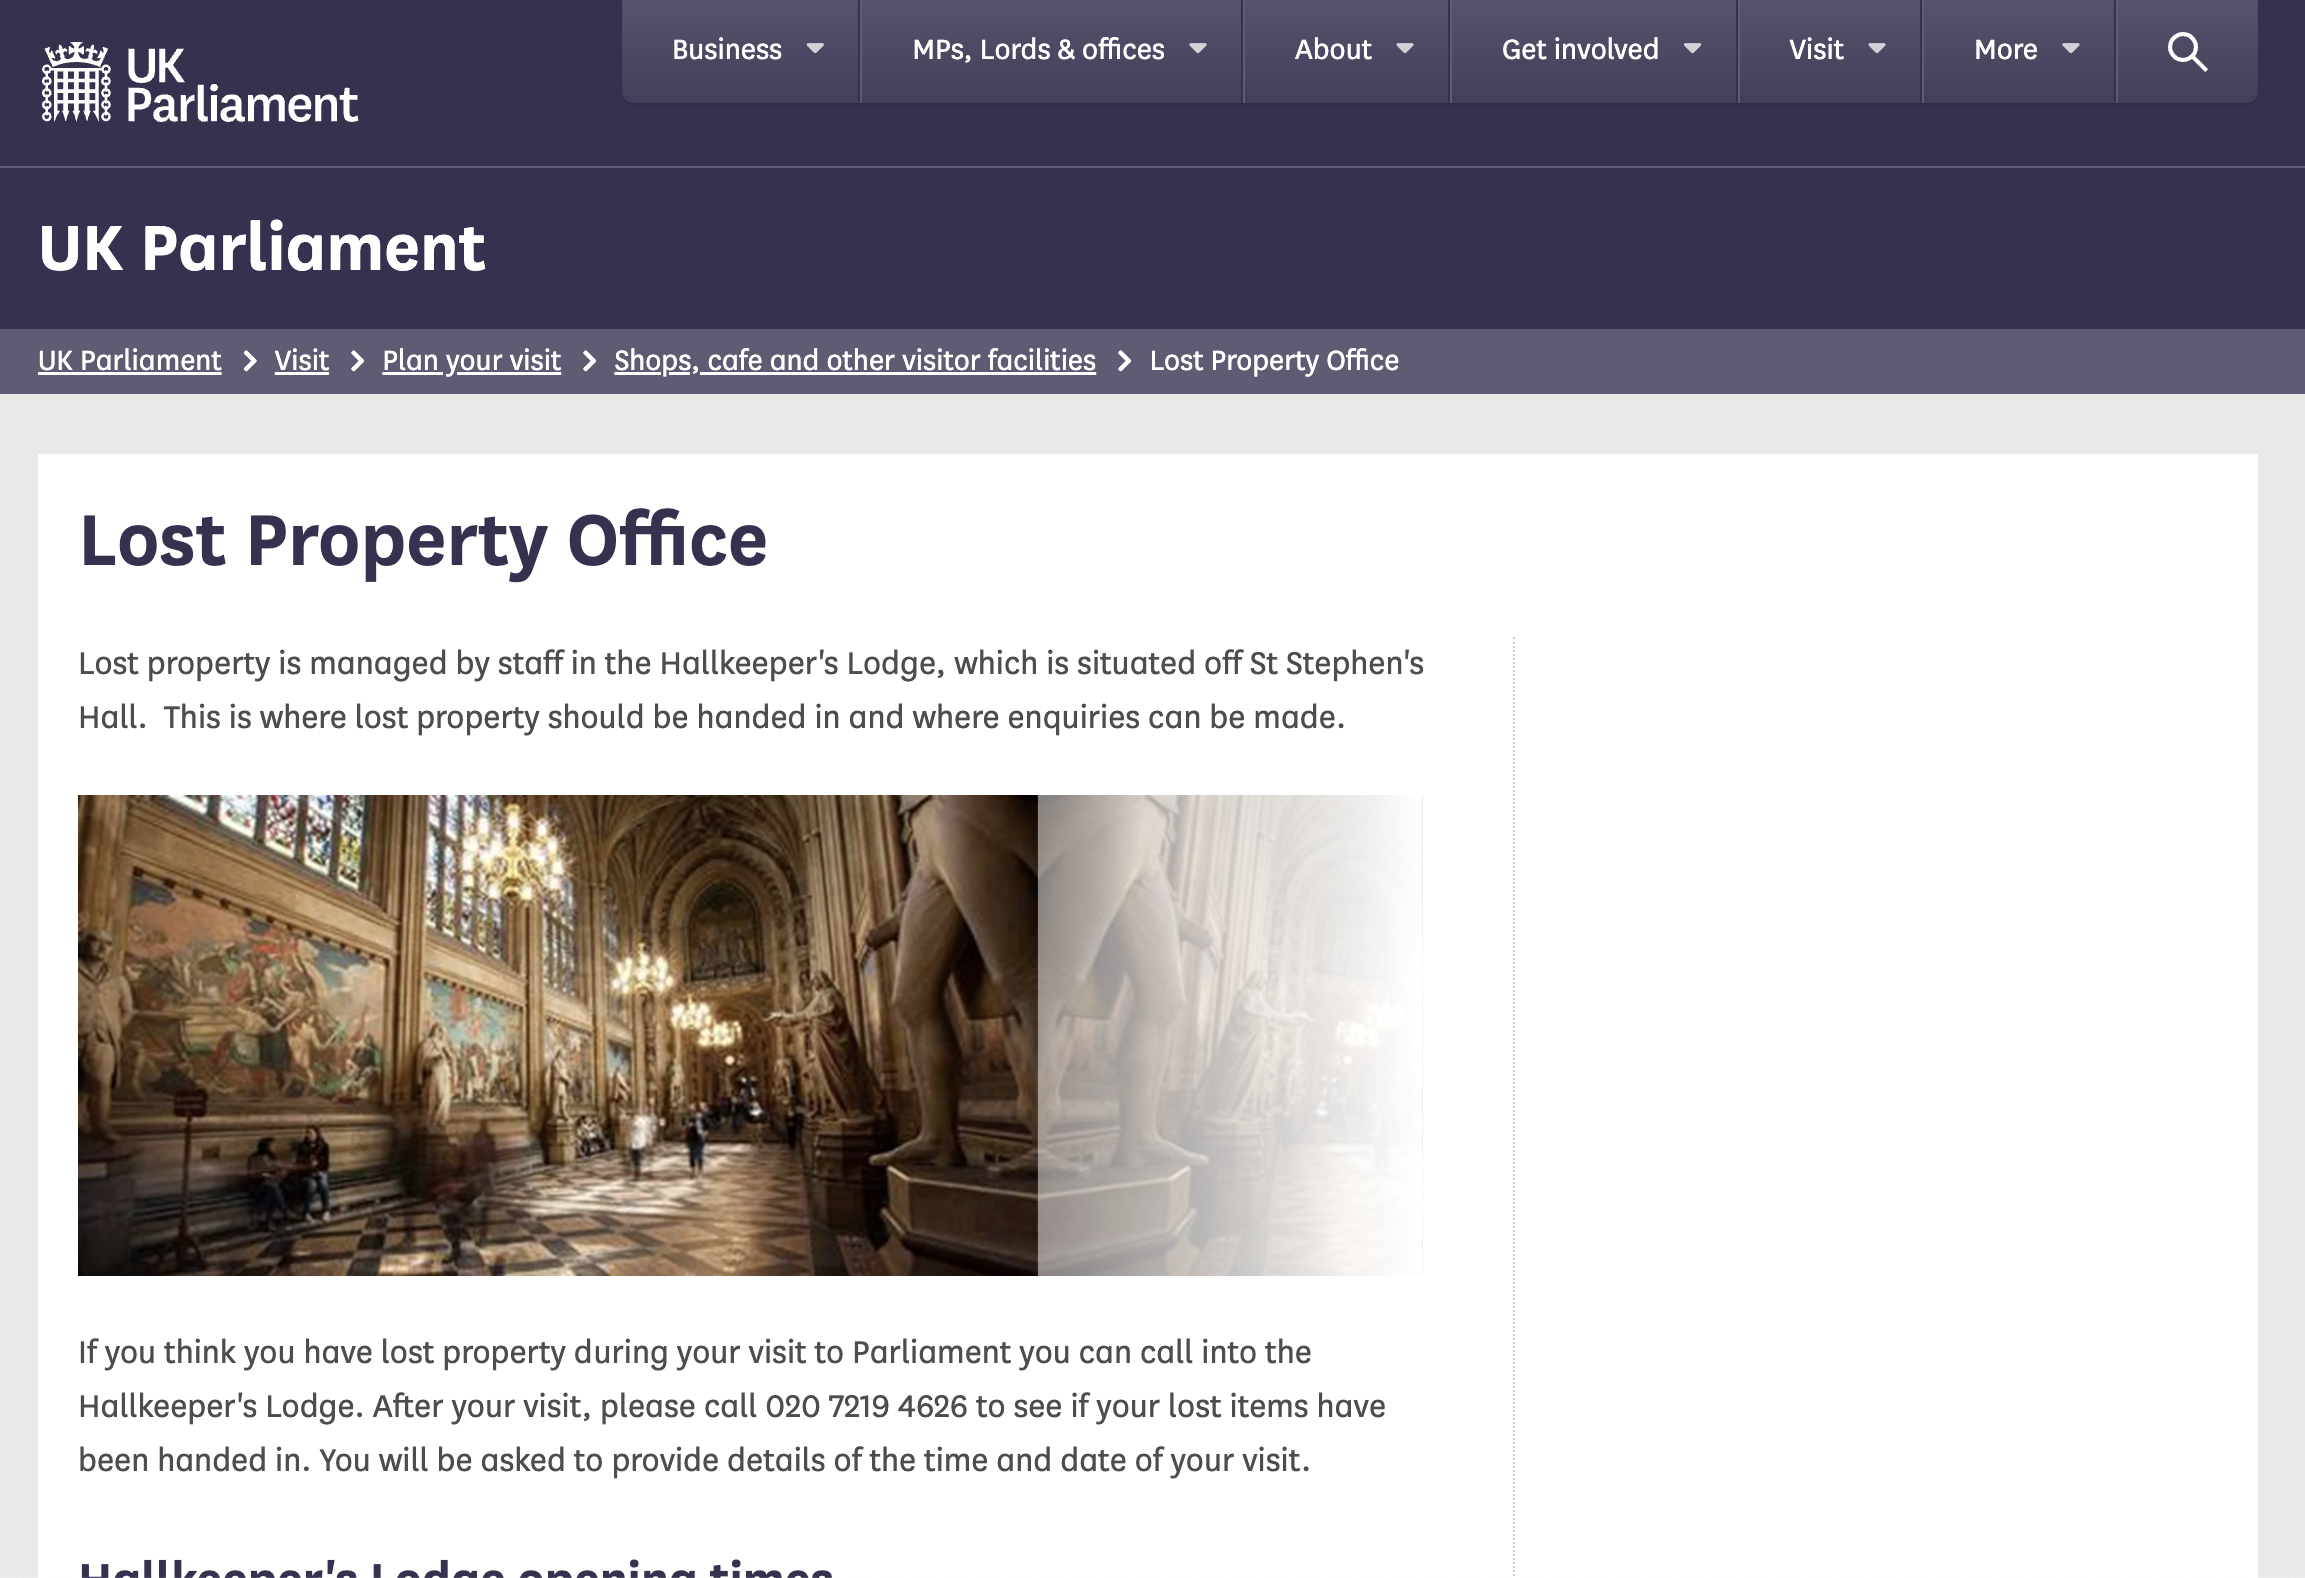
\includegraphics[width=.95\textwidth]{images/lostPropertyOffice}
	\parskip=6pt
	\caption{Скриншот системы <<Lost Property Office>>}
	\label{fig:lostPropertyOffice}
\end{figure}

На основании проведенного обзора можно сделать вывод, что существующие веб-сервисы и приложения для поиска и возврата утерянных вещей имеют некоторые преимущества, но также недостатки, которые ограничивают их функциональность и удобство использования. Веб-сервис Бюро находок будет разработан с учетом этих недостатков и предлагать более удобное взаимодействие между пользователями и сервисом.

Ниже приведена сравнительная таблица~\ref{tab:analogs_comparison} основных характеристик и функций приведенных выше аналогов:
\begin{table}[htb]
	\caption{Сравнительная таблица аналогов}
	\centering
	
	\tolerance=1
	\emergencystretch=10pt
	\hyphenpenalty=1
	\exhyphenpenalty=1
	\small
	\begin{tabular}{ |p{2cm}|p{3cm}|p{2cm}|p{2cm}|p{3cm}|p{2cm}| } 
		\hline
		Сервис~/ Приложение & Интерфейс и удобство использования & Опове\-ще\-ния & Точность определения местоположения & Регистрация и подача заявки & Доступ\-ность \\ \hline
		
		стол\-на\-ходок.рф & Простой и интуитивно понятный интерфейс & Отсут\-ству\-ют & Не\-оп\-ре\-де\-ле\-но & Простой процесс регистрации & Широкий доступ \\ \hline
		
		Find My Stuff & Простой и интуитивно понятный интерфейс & Опо\-ве\-ще\-ния через уведомления & Низкая точность & Простой процесс регистрации & Доступен только на смартфонах с GPS \\ \hline
		
		Lost Property Office & Неудобный процесс регистрации и подачи заявки & Отсут\-ству\-ют & Не\-оп\-ре\-де\-ле\-но & Неудобный процесс регистрации и подачи заявки & Огра\-ни\-чен\-ный доступ \\ \hline
	\end{tabular}
	\label{tab:analogs_comparison}
\end{table}

\subsection*{Вывод по разделу}

В аналитической части работы проведен детальный анализ существующих веб-ресурсов и приложений, предназначенных для поиска и возвращения утерянных вещей. Были изучены и проанализированы их функциональность, характеристики, преимущества и ограничения.

Одним из наиболее популярных и востребованных решений в данной сфере являются веб-сервисы и приложения "Бюро находок". Они предоставляют пользователям платформу для регистрации утерянных вещей и связи с их владельцами, что упрощает процесс поиска и возвращения потерянных предметов.


% Специальный раздел
\section{Специальный раздел}
\label{sec:special}

\subsection{Требования к разрабатываемой системе}

Требования к разрабатываемой системе представляют собой совокупность параметров и характеристик, которыми должно обладать разрабатываемое приложение для достижения поставленных целей и решения задач. Они определяют функциональность системы, ее поведение, а также условия, необходимые для ее корректной работы. Требования подразделяются на функциональные и нефункциональные.

Функциональные требования описывают специфические функции или действия, которые должна выполнять система. В контексте разрабатываемого приложения для поиска и возврата уянных вещей, это могут быть функции регистрации и авторизации пользователей, поиска утерянных вещей, добавления информации о утерянных вещах, связи между пользователями и системы уведомлений.

Нефункциональные требования определяют качественные характеристики системы, такие как производительность, безопасность, доступность, удобство использования, совместимость, масштабируемость, тестирование и документация.

Требования к разрабатываемой системе играют ключевую роль в процессе разработки приложения. Они служат основой для проектирования, реализации и тестирования системы. Без четко определенных требований невозможно разработать эффективное и надежное приложение, которое будет отвечать потребностям пользователей и бизнес-задачам.

В контексте курсовой работы на тему “Разработка приложения для поиска и возврата утерянных вещей”, требования к разрабатываемой системе позволяют сформулировать и структурировать задачи, которые должно решать приложение, а также определить параметры, необходимые для его успешной работы. Они служат основой для дальнейшего проектирования и разработки приложения, а также для оценки его эффективности и качества после внедрения.

\subsubsection{Функциональные требования}

\begin{enumerate}
	\item Приложение должно предоставлять возможность регистрации и авторизации пользователей.
	\item Приложение должно предоставлять возможность поиска утерянных вещей по различным критериям (например, по типу вещи, по месту утери и т.д.).
	\item Пользователи должны иметь возможность добавлять информацию о утерянных вещах, включая описание, фотографии и место утери.
	\item Приложение должно предоставлять функционал для связи между пользователем, который нашел вещь, и пользователем, который ее потерял.
	\item Приложение должно иметь систему уведомлений, которая будет информировать пользователей о новых найденных вещах, соответствующих их критериям поиска.
\end{enumerate}

В соответствии с требованиями была составлена ER-диаграмма, которая представлена на рис.~\ref{fig:erd}. Пользователь регистрируется посредством OAuth, при этом заполняются таблицы Account и User. Пользователь заполняет свои социальные сети UserSocialNetwork. Пользователь заполняет форму с потерянной или найденной вещью в LostAndFoundItem, и привязывает к карточки вещи соц. сети, по которой с ним можно связаться.

\begin{figure}[htb]
	\centering
	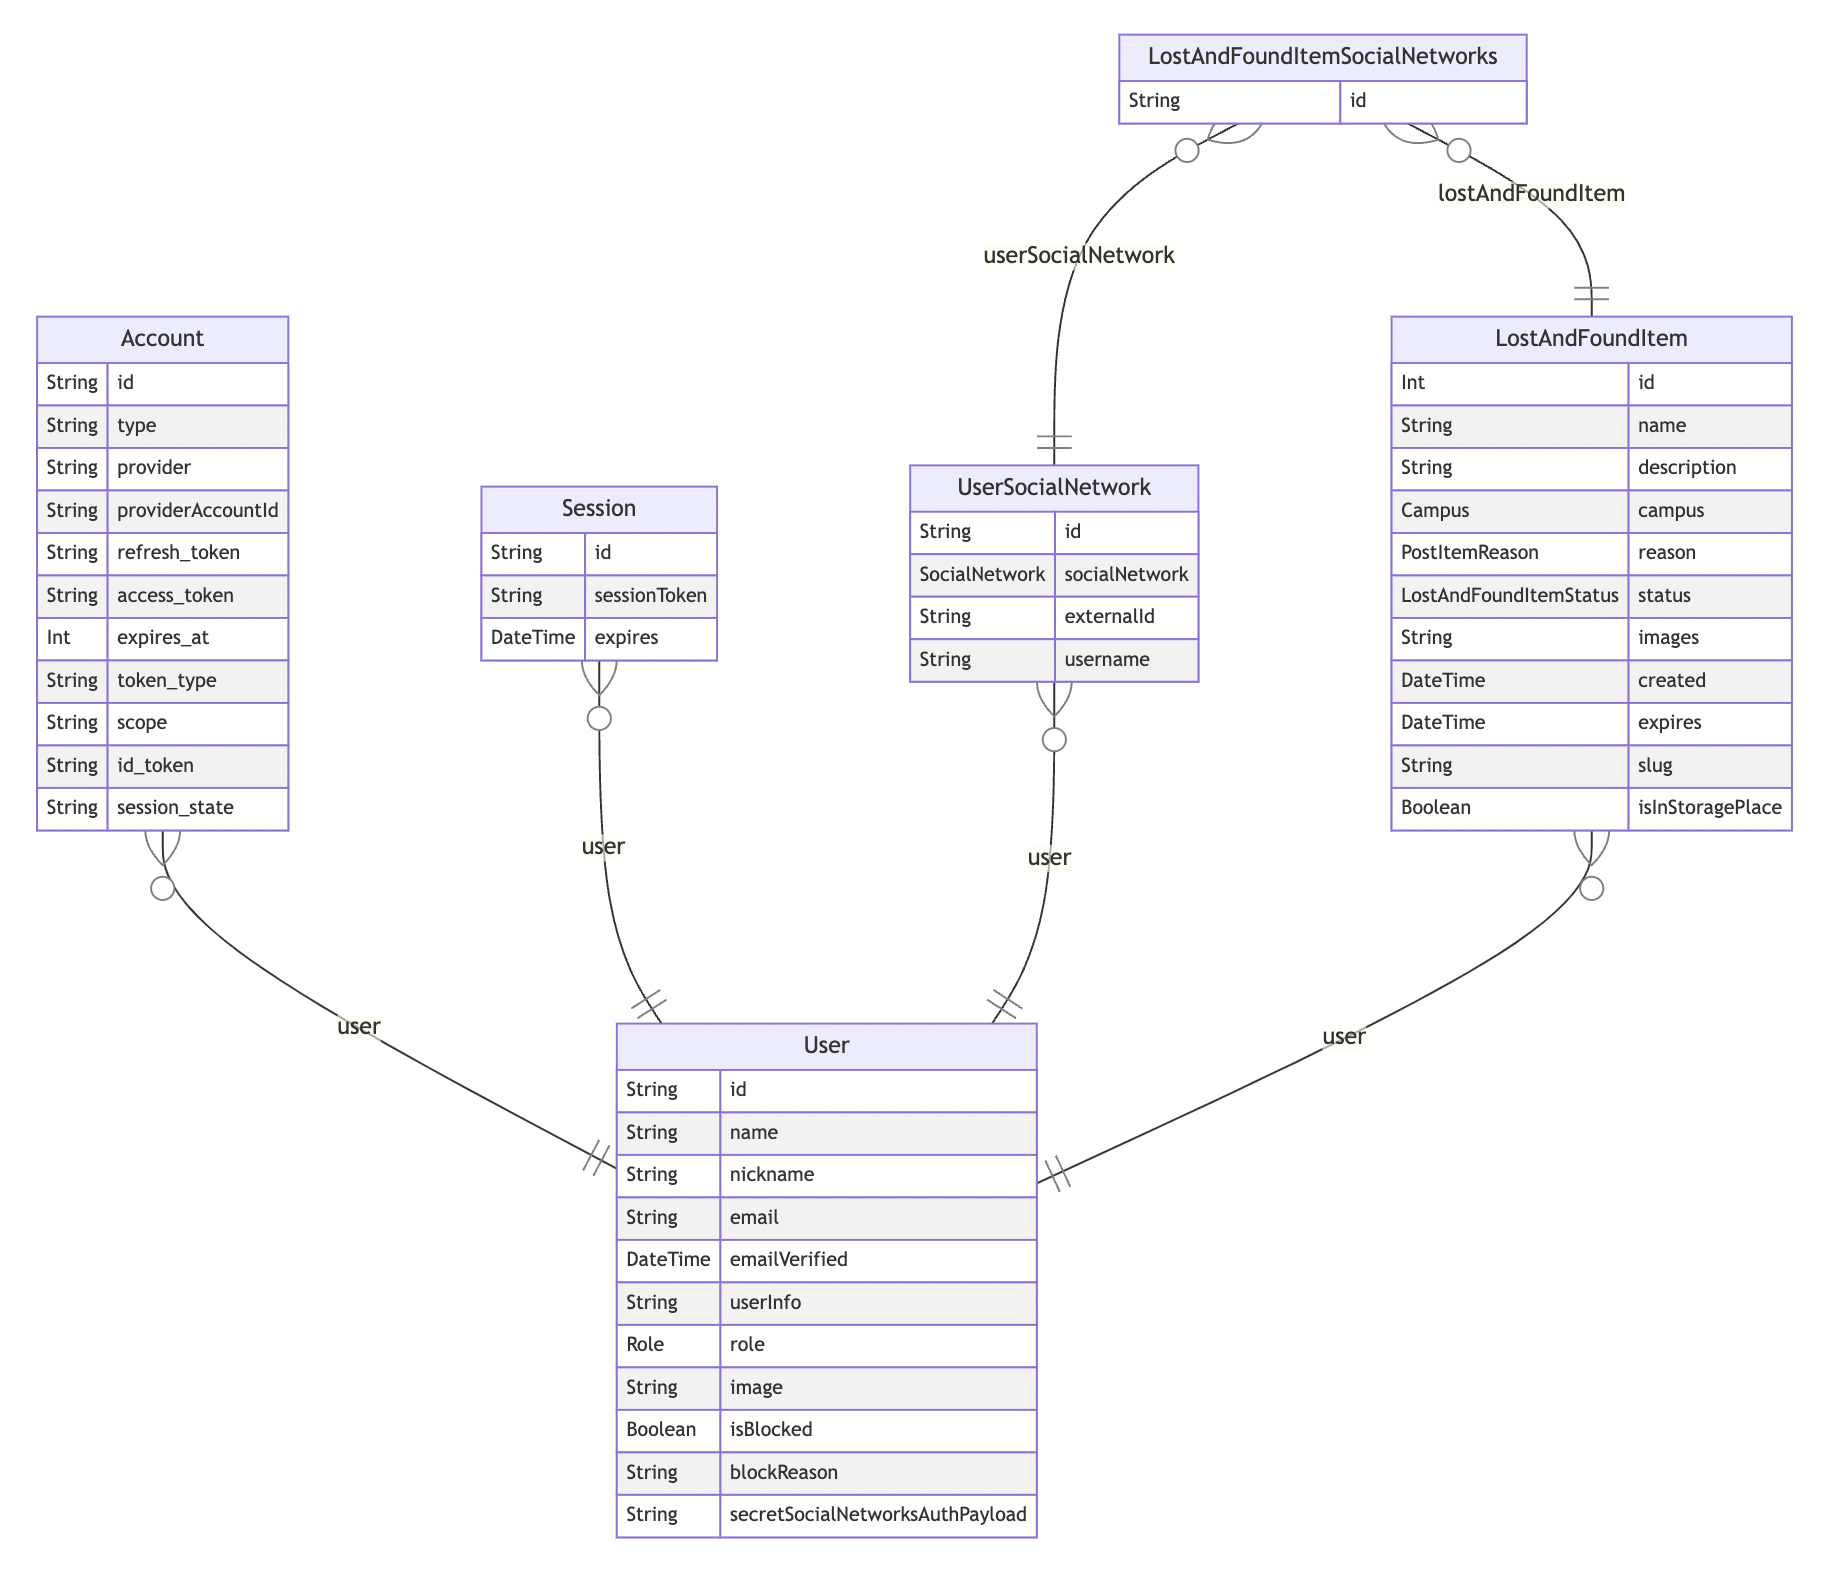
\includegraphics[width=.95\textwidth]{images/erd}
	\parskip=6pt
	\caption{ER-диаграмма системы}
	\label{fig:erd}
\end{figure}

\subsubsection{Нефункциональные требования}

\begin{enumerate}
	\item Приложение должно обеспечивать быстрый поиск и отображение результатов, а также быстрое добавление информации о утерянных вещах.
	\item Все данные пользователей должны быть защищены.
	\item Приложение должно быть доступно для использования 24/7.
	\item Интерфейс приложения должен быть интуитивно понятным и удобным для пользователей разного уровня компьютерной грамотности.
	\item Приложение должно быть совместимо с основными операционными системами (iOS, Android) и браузерами (Chrome, Firefox, Safari, Edge).
	\item Приложение должно быть способно обслуживать большое количество пользователей одновременно без снижения производительности.
	\item Приложение должно быть тщательно протестировано на наличие ошибок и уязвимостей перед запуском.
\end{enumerate}

Клиентское приложение работает в вебе, использует кросс-платформенные технологии (JS, HTML, CSS). Защита пользователя возложено на независимый сервер авторизации.

\subsection{Проектирование модулей автоматизации процессов}

Проектирование модулей автоматизации процессов включает в себя разработку структуры и функционала модулей, которые будут автоматизировать ключевые процессы приложения для поиска и возврата утерянных вещей. В данном случае, ключевыми процессами являются: регистрация и авторизация пользователей, добавление и поиск утерянных вещей, связь между пользователями и система уведомлений.

\begin{figure}[htb]
	\centering
	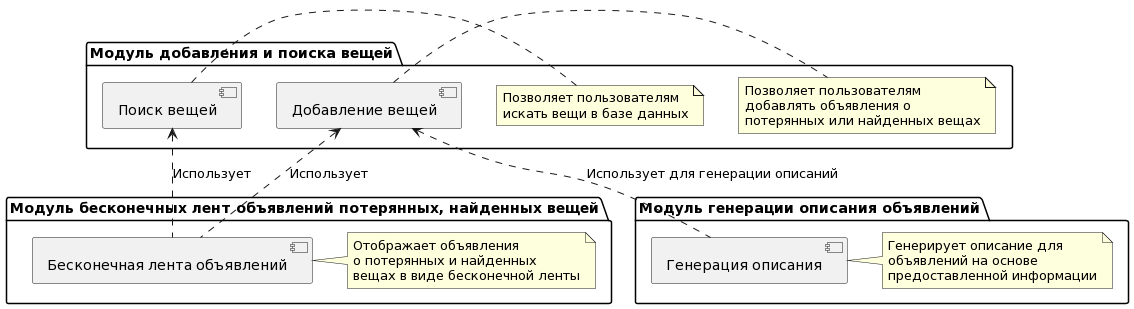
\includegraphics[width=.9\textwidth]{images/full-diagram.png}
	\parskip=6pt
	\caption{Диаграмма компонентов системы}
	\label{fig:агддВшфпкфь}
\end{figure}

\begin{comment}
@startuml
package "Модуль бесконечных лент объявлений потерянных, найденных вещей" {
	[Бесконечная лента объявлений] as InfiniteScroll
	note right of InfiniteScroll : Отображает объявления\nо потерянных и найденных\nвещах в виде бесконечной ленты
}

package "Модуль добавления и поиска вещей" {
	[Добавление вещей] as AddItems
	[Поиск вещей] as SearchItems
	note right of AddItems : Позволяет пользователям\nдобавлять объявления о\nпотерянных или найденных вещах
	note right of SearchItems : Позволяет пользователям\nискать вещи в базе данных
}

package "Модуль генерации описания объявлений" {
	[Генерация описания] as DescriptionGeneration
	note right of DescriptionGeneration : Генерирует описание для\nобъявлений на основе\nпредоставленной информации
}

'Relations
InfiniteScroll .up.> AddItems : Использует
InfiniteScroll .up.> SearchItems : Использует
DescriptionGeneration .up.> AddItems : Использует для генерации описаний
@enduml
\end{comment}

\subsubsection{Модуль регистрации и авторизации пользователей}

Этот модуль предназначен для создания и поддержки учетных записей пользователей. Он должен включать функции регистрации, авторизации через сервер посредника (сервер авторизации РТУ МИРЭА).


\begin{figure}[htb]
	\centering
	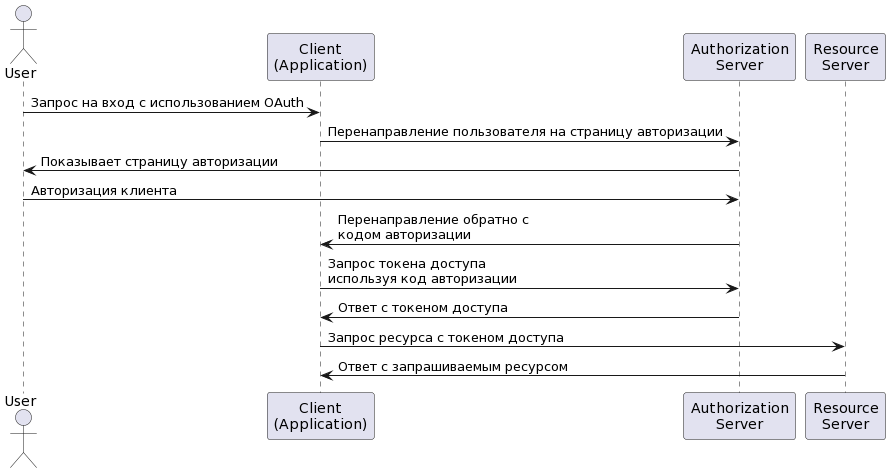
\includegraphics[width=.9\textwidth]{images/registation-diagram.png}
	\parskip=6pt
	\caption{Диаграмма последовательностей авторизации}
	\label{fig:authDiagram}
\end{figure}

\begin{comment}
@startuml
actor User as user
participant "Client\n(Application)" as client
participant "Authorization\nServer" as auth
participant "Resource\nServer" as resource

user -> client: Запрос на вход с использованием OAuth
client -> auth: Перенаправление пользователя на страницу авторизации
auth -> user: Показывает страницу авторизации
user -> auth: Авторизация клиента
auth -> client: Перенаправление обратно с\nкодом авторизации
client -> auth: Запрос токена доступа\nиспользуя код авторизации
auth -> client: Ответ с токеном доступа
client -> resource: Запрос ресурса с токеном доступа
resource -> client: Ответ с запрашиваемым ресурсом
@enduml
\end{comment}


\subsubsection{Модуль бесконечных лент объявлений потерянных, найденных вещей}

Модуль бесконечных лент объявлений представляет собой ключевой элемент приложения для поиска и возврата утерянных вещей. Он предназначен для отображения объявлений о потерянных и найденных вещах в формате бесконечной ленты, обеспечивая пользователю удобный и непрерывный доступ к информации.

\begin{figure}[htb]
	\centering
	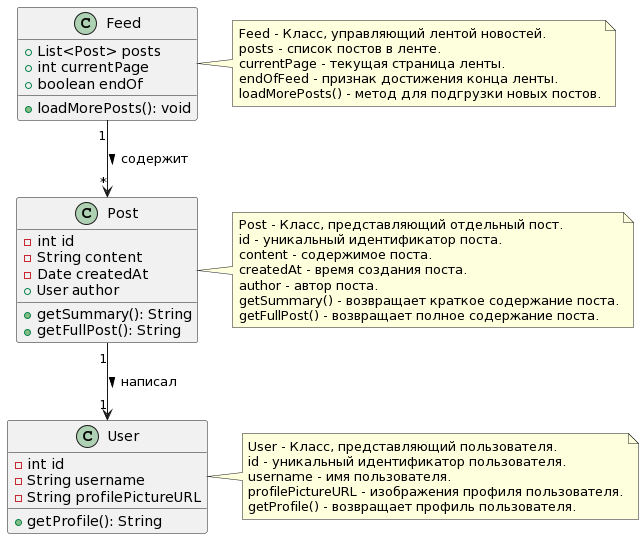
\includegraphics[width=.9\textwidth]{images/feed-diagram.png}
	\parskip=6pt
	\caption{Диаграмма классов бесконечной ленты}
	\label{fig:feedDiagram}
\end{figure}

\begin{comment}
@startuml
class Feed {
	+List<Post> posts
	+int currentPage
	+boolean endOf
	+loadMorePosts(): void
}

class Post {
	-int id
	-String content
	-Date createdAt
	+User author
	+getSummary(): String
	+getFullPost(): String
}

class User {
	-int id
	-String username
	-String profilePictureURL
	+getProfile(): String
}

Feed "1" --> "*" Post : содержит >
Post "1" --> "1" User : написал >

note right of Feed
Feed - Класс, управляющий лентой новостей.
posts - список постов в ленте.
currentPage - текущая страница ленты.
endOfFeed - признак достижения конца ленты.
loadMorePosts() - метод для подгрузки новых постов.
end note

note right of Post
Post - Класс, представляющий отдельный пост.
id - уникальный идентификатор поста.
content - содержимое поста.
createdAt - время создания поста.
author - автор поста.
getSummary() - возвращает краткое содержание поста.
getFullPost() - возвращает полное содержание поста.
end note

note right of User
User - Класс, представляющий пользователя.
id - уникальный идентификатор пользователя.
username - имя пользователя.
profilePictureURL - изображения профиля пользователя.
getProfile() - возвращает профиль пользователя.
end note
@enduml
\end{comment}

\subsubsection{Модуль добавления и поиска вещей}

Этот модуль отвечает за добавление информации о утерянных вещах в базу данных и поиск по этой базе. Он должен предоставлять пользователю возможность добавлять описание, фотографии и место утери вещи, а также осуществлять поиск по различным критериям.

\begin{figure}[htb]
	\centering
	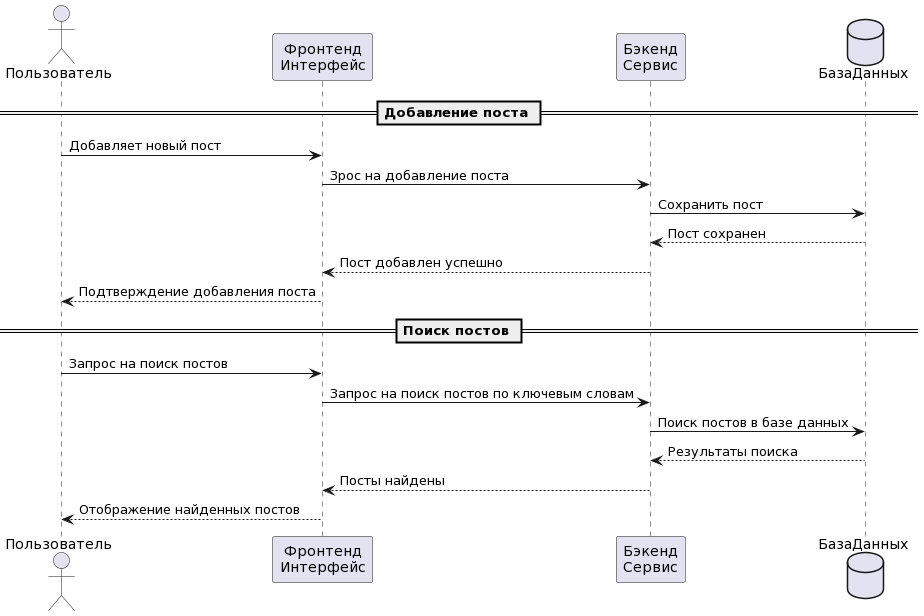
\includegraphics[width=.9\textwidth]{images/seach-diagram.png}
	\parskip=6pt
	\caption{Диаграмма последовательностей добавления и поиска вещей}
	\label{fig:searchDiagram}
\end{figure}

\begin{comment}
@startuml
actor Пользователь as User
participant "Фронтенд\nИнтерфейс" as Frontend
participant "Бэкенд\nСервис" as Backend
database БазаДанных as Database

== Добавление поста ==
User -> Frontend : Добавляет новый пост
Frontend -> Backend : Запрос на добавление поста
Backend -> Database : Сохранить пост
Database --> Backend : Пост сохранен
Backend --> Frontend : Пост добавлен успешно
Frontend --> User : Подтверждение добавления поста

== Поиск постов ==
User -> Frontend : Запрос на поиск постов
Frontend -> Backend : Запрос на поиск постов по ключевым словам
Backend -> Database : Поиск постов в базе данных
Database --> Backend : Результаты поиска
Backend --> Frontend : Посты найдены
Frontend --> User : Отображение найденных постов
@enduml
\end{comment}

\begin{figure}[htb]
	\centering
	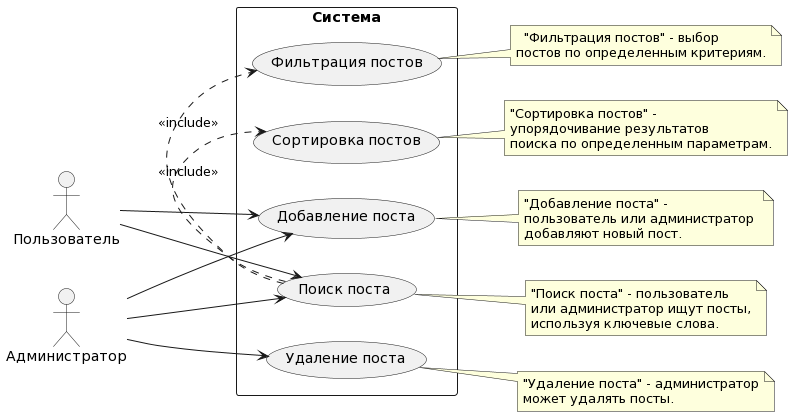
\includegraphics[width=.9\textwidth]{images/seach-diagram-2.png}
	\parskip=6pt
	\caption{Диаграмма вариантов использования добавления и поиска вещей}
	\label{fig:searchDiagram2}
\end{figure}

\begin{comment}
@startuml
left to right direction
actor Пользователь
actor Администратор

rectangle Система {
	Пользователь --> (Добавление поста)
	Пользователь --> (Поиск поста)
	Администратор --> (Добавление поста)
	Администратор --> (Поиск поста)
	Администратор --> (Удаление поста)
	(Поиск поста) .> (Фильтрация постов) : <<include>>
	(Поиск поста) .> (Сортировка постов) : <<include>>
}

note right of (Добавление поста)
"Добавление поста" - 
пользователь или администратор 
добавляют новый пост.
end note

note right of (Поиск поста)
"Поиск поста" - пользователь 
или администратор ищут посты,
используя ключевые слова.
end note

note right of (Удаление поста)
"Удаление поста" - администратор
может удалять посты.
end note

note right of (Фильтрация постов)
"Фильтрация постов" - выбор
постов по определенным критериям.
end note

note right of (Сортировка постов)
"Сортировка постов" - 
упорядочивание результатов 
поиска по определенным параметрам.
end note
@enduml
\end{comment}

\subsubsection{Модуль генерации описания объявлений}

Модуль генерации описания объявлений является важным компонентом приложения для поиска и возврата утерянных вещей. Он предназначен для автоматического создания описаний объявлений на основе введенных пользователем данных, что облегчает процесс создания объявлений и повышает их качество.

\begin{figure}[htb]
	\centering
	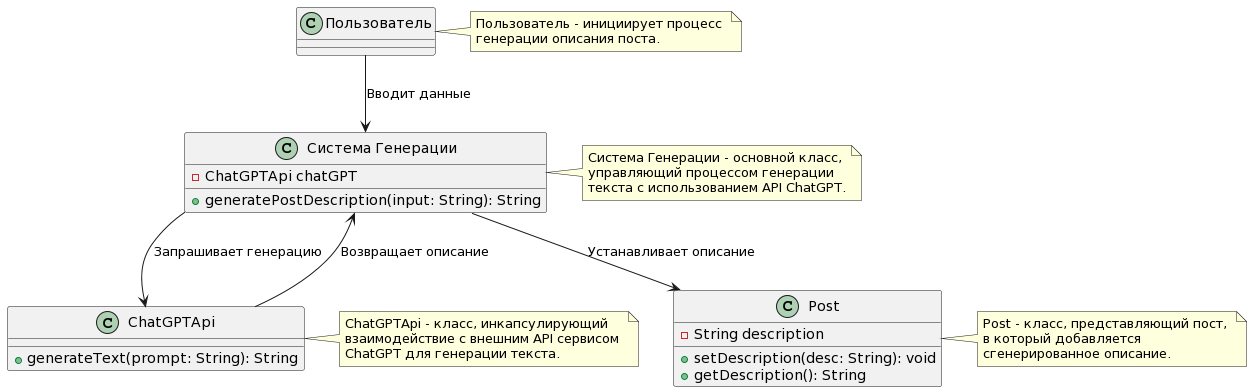
\includegraphics[width=.95\textwidth]{images/generating-diagram.png}
	\parskip=6pt
	\caption{Диаграмма классов генеарации описания вещей}
	\label{fig:generatingDiagram}
\end{figure}

\begin{comment}
@startuml
class "Пользователь" as User {
}

class "Система Генерации" {
	-ChatGPTApi chatGPT
	+generatePostDescription(input: String): String
}

class "ChatGPTApi" {
	+generateText(prompt: String): String
}

class "Post" {
	-String description
	+setDescription(desc: String): void
	+getDescription(): String
}

User --> "Система Генерации" : Вводит данные
"Система Генерации" --> ChatGPTApi : Запрашивает генерацию
ChatGPTApi --> "Система Генерации" : Возвращает описание
"Система Генерации" --> Post : Устанавливает описание

note right of User
Пользователь - инициирует процесс 
генерации описания поста.
end note

note right of "Система Генерации"
Система Генерации - основной класс, 
управляющий процессом генерации 
текста с использованием API ChatGPT.
end note

note right of ChatGPTApi
ChatGPTApi - класс, инкапсулирующий 
взаимодействие с внешним API сервисом 
ChatGPT для генерации текста.
end note

note right of Post
Post - класс, представляющий пост, 
в который добавляется 
сгенерированное описание.
end note
@enduml
\end{comment}

\subsection*{Вывод по разделу}

Проектирование модулей автоматизации процессов является важным этапом в разработке приложения для поиска и возврата утерянных вещей. Каждый из модулей, включая модуль регистрации и авторизации пользователей, модуль бесконечных лент объявлений, модуль добавления и поиска утерянных вещей и модуль генерации описания объявлений, играет свою уникальную роль в обеспечении функциональности приложения.

Каждый из этих модулей важен для обеспечения удобства использования приложения, и их совместная работа позволяет создать надежное и функциональное приложение для поиска и возврата утерянных вещей.

% Технологический раздел
\section{Технологический раздел}
\label{sec:technology}

\subsection{Выбор технологий для реализации системы}

TODO

\subsection{Реализация модулей автоматизации процессов}

TODO

\subsubsection{Модуль бесконечных лент объявлений потерянных, найденных вещей}

TODO

\subsubsection{Модуль полнотекстового поиска объявлений}

TODO

\subsubsection{Модуль генерации описания объявлений}

TODO

\subsection*{Вывод по разделу}

TODO

% Экономический раздел
\section{Экономический раздел}
\label{sec:economy}

\subsection{Планирование разработки системы}

Основой данной выпускной квалификационной работы является <<Разработка системы для поиска и возврата утерянных вещей>>. В данном разделе определяются уровень сложности и затраты на создание программного и аппаратного обеспечения, а также оценивается экономическая выгода, которую можно получить от использования разрабатываемого программного обеспечения.

\subsubsection{Определение трудоемкости и продолжительности работ по созданию УСПД}

В этом разделе определяются уровень сложности и затраты на создание программного и аппаратного обеспечения, а также проводится оценка экономической выгоды от использования разрабатываемого ПО. Процесс разработки включает анализ предметной области, имитационный анализ, создание, настройку и тестирование системы.

\begin{itemize}	
	\item Техническое задание. Регламентированы следующие этапы исследования: составление технического задания, включающего формулировку задач, подбор литературы, сбор исходных данных, определение системных требований, а также определение этапов, фаз и сроков разработки программного обеспечения.
	
	\item Эскизный проект. Этот этап включает в себя использование программных средств для анализа схожих тем, разработки общих программных структур и структур по подсистемам, создания прототипов и документации.
	
	\item Технический проект. Этот этап включает в себя определение требований к программному обеспечению и выбор инструментов и использование программных средств.
	
	\item Рабочий проект. Этап включает компоновку и дизайн, программирование, тестирование и отладку ПО, проектирование плат, а также координацию и утверждение работоспособности всей системы.
	
	\item Внедрение. Подразумевает под собой использование на реальной инфраструктуре; анализ полученных данных в результате исследований, благодаря которым можно будет скорректировать техническую документацию.
\end{itemize}

Трудоемкость работ по созданию программного обеспечения носит вероятностный характер, поскольку определяется суммой сложности этапов и видов работ, оцениваемых экспертами в ручные дни, и зависит от многих факторов, которые трудно учесть.

Трудоемкость каждого вида работ определяется по формуле~(\ref{eq:t_i}).
\begin{equation}\label{eq:t_i}
	t_i=\frac{3 \cdot t_{min} + 2 \cdot t_{max}}{5},
\end{equation}
где $t_{min}$~--- минимально возможная трудоемкость выполнения отдельного вида работ; \\
$t_{max}$~--- максимально возможная трудоемкость выполнения отдельного вида
работ.

Различные виды работ имеют свою продолжительность в календарных днях ($T_{i}$), определяясь по формуле~(\ref{eq:T_i}), в днях:
\begin{equation}\label{eq:T_i}
	T_i=\frac{t_{i}}{\text{Ч}_{i}} \cdot K_{\text{вых}},
\end{equation}
где $t_{i}$~--- трудоемкость работ, человеко-дней; \\
$\text{Ч}_{i}$~--- численность исполнителей, человек; \\
$K_{\text{вых}}$~--- коэффициент, учитывающий выходные и праздничные дни, находится по формуле~(\ref{eq:k_vih}):
\begin{equation}\label{eq:k_vih}
	K_{\text{вых}}=\frac{K_{\text{кал}}}{K_{\text{раб}}},
\end{equation}
где $K_{\text{кал}}$~--- календарные дни; \\
$K_{\text{раб}}$~--- рабочие дни; \\
$K_{\text{вых}}$~--- 1,48.

Далее предоставляется перечень разновидностей и стадий рабочей деятельности по разработке ПО, экспертные оценки, а также рассчитываемые переменные их трудоемкости, а также продолжительность каждого вида работ, рассчитанные по формулам~(\ref{eq:t_i}) и~(\ref{eq:T_i}), представлены в таблице~\ref{tab:work_hours}.

\begin{longtable}{ |x{1cm}|x{3cm}|x{1cm}|x{1cm}|x{1cm}|x{3cm}|x{3cm}| } 
	
	\caption{Расчет трудоемкости и продолжительности работ по созданию ПО и аппаратных средств календарных дней}
	\label{tab:work_hours} \\ 
	
	\hline 
	\parbox[t]{2mm}{\multirow{2}{*}{\rotatebox[origin=c]{90}{\bfseries \textnumero{} работы\hspace{5mm}}}} &
	\multicolumn{1}{p{3cm}|}{\multirow{2}{*}{\parbox{3cm}{\bfseries Стадии разработки}}} & 
	\multicolumn{3}{p{3cm}|}{\bfseries Трудоемкость, чел. дни} & 
	\multicolumn{1}{p{3cm}|}{\bfseries Количество работников, чел.} & 
	\multicolumn{1}{p{3cm}|}{\bfseries Про\-дол\-жи\-тель- ность работ, календарные дни}
	
	\endfirsthead
	
	
	\multicolumn{7}{l}{{Продолжение таблицы \thetable{}.}} \\ \hline
	\parbox[t]{2mm}{\multirow{2}{*}{\rotatebox[origin=c]{90}{\bfseries \textnumero{} работы\hspace{5mm}}}} &
	\multicolumn{1}{p{3cm}|}{\multirow{2}{*}{\parbox{3cm}{\bfseries Стадии разработки}}} & 
	\multicolumn{3}{p{3cm}|}{\bfseries Трудоемкость, чел. дни} & 
	\multicolumn{1}{p{3cm}|}{\bfseries Количество работников, чел.} & 
	\multicolumn{1}{p{3cm}|}{\bfseries Про\-дол\-жи\-тель- ность работ, календарные дни}
	\endhead
	
	\endfoot
	
	\endlastfoot
	
	\hline
	
	&& $t_{min}$ & $t_{max}$ & $t_{i}$ & $\text{Ч}_i$ & $T_i$ \\ \hline
	
	\multicolumn{7}{|c|}{Техническое задание} \\ \hline
	
	1 & - постановка задачи & 3 & 6 & 4.2 & 1 & 6.2 \\ \hline
	
	2 & - подбор литературы & 2 & 3 & 2.4 & 1 & 3.6 \\ \hline
	
	3 & - сбор исходных данных & 4 & 5 & 4.4 & 1 & 6.5 \\ \hline
	
	4 & - определение требований к системе & 3 & 4 & 3.4 & 1 & 5.0 \\ \hline
	
	5 & - определение стадий, этапов и сроков разработки ПО & 2 & 3 & 2.4 & 1 & 3.6 \\ \hline
	
	\multicolumn{7}{|c|}{Эскизный проект} \\ \hline
	
	6 & - анализ программных средств схожей тематики & 7 & 8 & 7.4 & 1 & 11.0 \\ \hline
	
	7 & - разработка общей структуры ПО & 4 & 8 & 5.6 & 1 & 8.3 \\ \hline
	
	8 & - разработка структуры программы и подсистем & 5 & 8 & 6.2 & 1 & 9.2 \\ \hline
	
	9 & - создание прототипа & 4 & 6 & 4.8 & 1 & 7.1 \\ \hline
	
	10 & - документирование & 2 & 3 & 2.4 & 1 & 3.6 \\ \hline
	
	11 & - определение требований к ПО & 3 & 4 & 3.4 & 1 & 5.0 \\ \hline
	
	12 & - выбор инструментальных средств & 3 & 4 & 3.4 & 1 & 5.0 \\ \hline
	
	\multicolumn{7}{|c|}{Рабочий проект} \\ \hline
	
	13 & - программирование & 20 & 25 & 22 & 1 & 32.6 \\ \hline
	
	14 & - тестирование и отладка ПО & 7 & 8 & 7.4 & 1 & 11.0 \\ \hline
	
	15 & - разработка программной документации & 4 & 6 & 4.8 & 1 & 7.1 \\ \hline
	
	16 & - согласование и утверждение работоспособности системы & 2 & 3 & 2.4 & 1 & 3.6 \\ \hline
	
	\multicolumn{7}{|c|}{Внедрение} \\ \hline
	
	17 & - опытная эксплуатация & 6 & 8 & 6.8 & 1 & 10.1 \\ \hline
	
	18 & - анализ данных, полученных в результате эксплуатации & 2 & 4 & 2.8 & 1 & 4.1 \\ \hline
	
	19 & - корректировка технической документации по результатам испытаний & 1 & 2 & 1.4 & 1 & 2.1 \\ \hline
	
	& {\bfseries Общая трудоемкость разработки} &&& 98 && 144 \\ \hline
\end{longtable}

Следовательно, общая продолжительность проведения работ $T_{i} = 144$.

\subsubsection{Построение ленточного графика проведения исследования}

В качестве инструмента планирования используется ленточный график~(\ref{fig:work_waterfall}).
\begin{figure}[H]
	\centering
	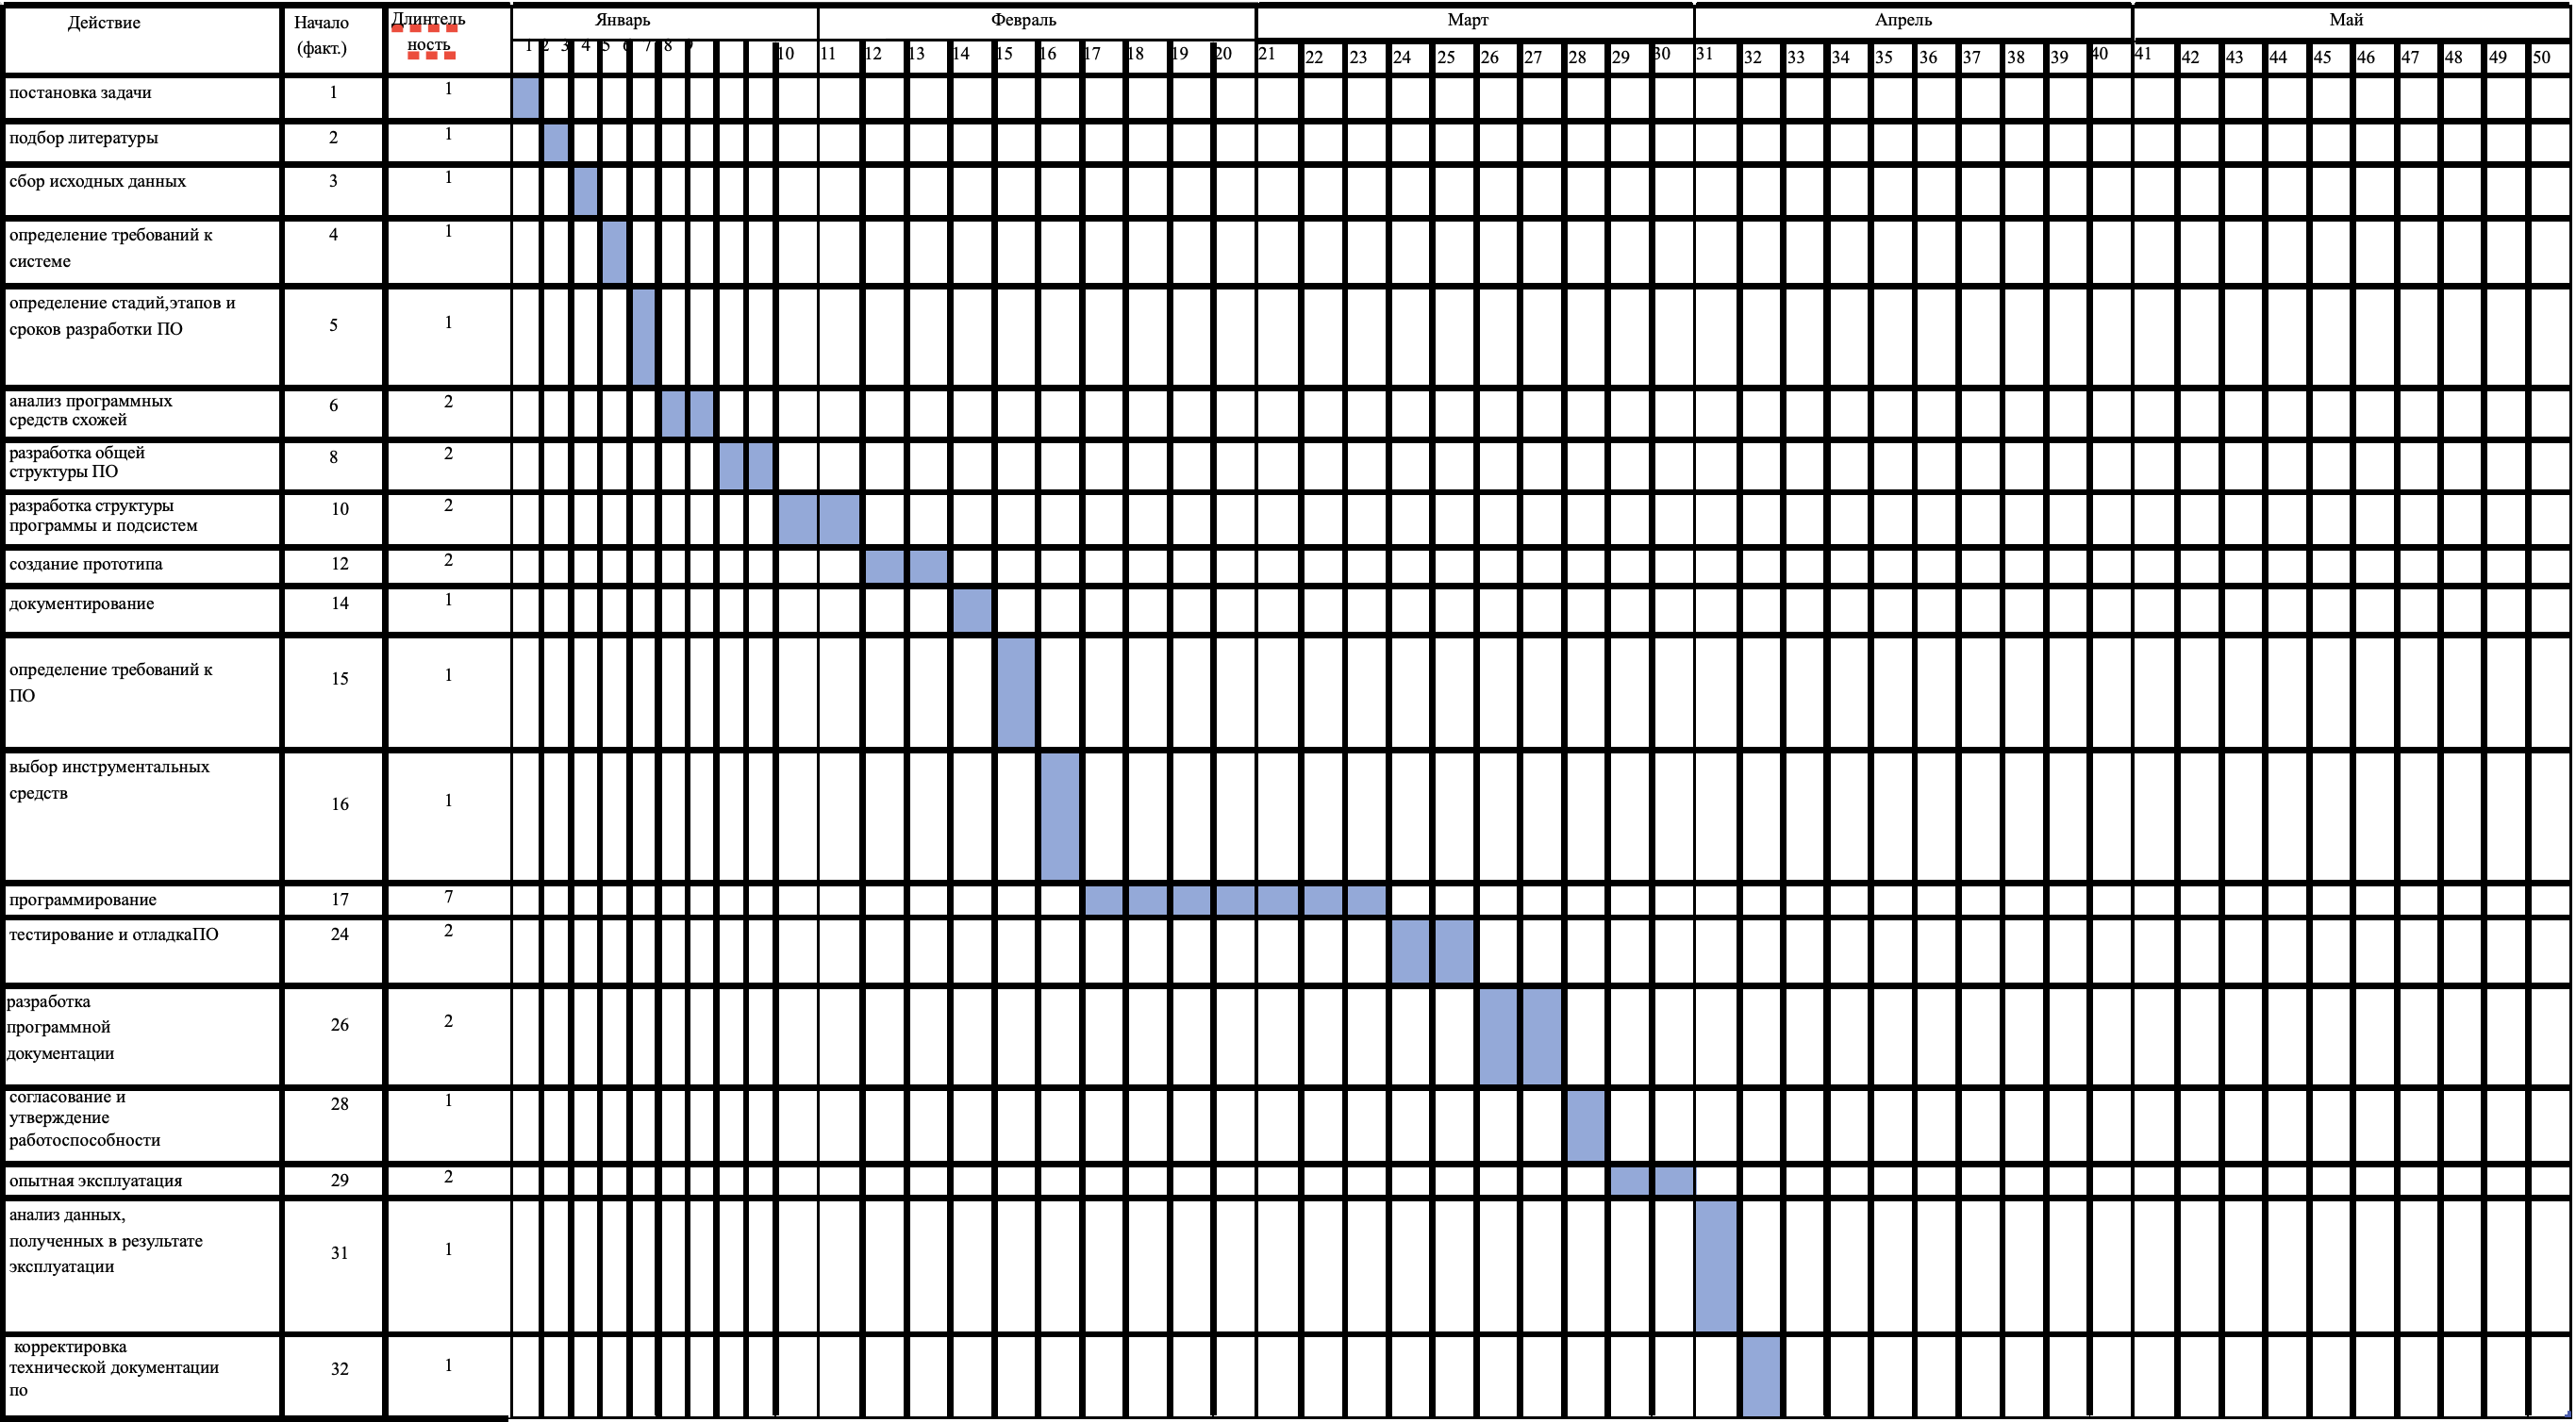
\includegraphics[width=.7\textheight,angle=90,origin=c]{images/work_waterfall}
	\parskip=6pt
	\caption{Ленточный график}
	\label{fig:work_waterfall}
\end{figure}

Подобный график позволяет наглядно представить логическую
последовательность и взаимосвязь отдельных работ. График представляет собой
таблицу с перечислением названий стадий разработки, видов работ, длительность выполнения работ. Данный график построен по данным таблицы~\ref{tab:work_hours}. В этом графике временная единица выполнения работ оценивается в 3 дня.

\subsection{Расчет сметы затрат на разработку представленной работы}

Сметная стоимость проектирования и внедрения программы включает в себя затраты, определяемые по формуле~(\ref{eq:estimate}):
\begin{equation}\label{eq:estimate}
	C_{\text{пр}} = C_{\text{осн}} + C_{\text{доп}} + C_{\text{соц}} + C_{\text{м}} + C_{\text{маш.вр}} + C_{\text{н}},
\end{equation}
где $C_{\text{пр}}$~--- стоимость разработки ПО; \\
$C_{\text{осн}}$~--- основная заработная плата исполнителей; \\
$C_{\text{доп}}$~--- дополнительная заработная плата исполнителей, учитывающая потери времени на отпуска и болезни (принимается в среднем 10\% от основной заработной платы; \\
$C_{\text{соц}}$~--- отчисления в фонд социального страхования – 30\% от основной и дополнительной заработной платы; \\
$C_{\text{м}}$~--- затраты на используемые материалы; \\
$C_{\text{маш.вр}}$~--- стоимость машинного времени; \\
$C_{\text{н}}$~--- накладные расходы включают затраты на управление, уборку, ремонт, электроэнергию, отопление и др. (принимаются в размере 60\% от основной и дополнительной заработной платы).

\subsubsection{Основная заработная плата исполнителей}

На статью «Заработная плата» относят заработную плату научных, инженерно-технических и других работников, непосредственно участвующих в разработке ПО. Расчет ведется по формуле (\ref{eq:salary}):

\begin{equation}\label{eq:salary}
	\text{З}_{\text{исп}} = \text{З}_{\text{ср}} \cdot T,
\end{equation}
где $\text{З}_{\text{исп}}$~--- заработная плата исполнителей (руб.); \\
$\text{З}_{\text{ср}}$~--- средняя тарифная ставка работника организации разработчика ПО (руб./чел./дни); \\
$T$~--- трудоемкость разработки ПО (чел.дни).

$\text{З}_{\text{ср}}$ определяется по формуле~(\ref{eq:work_tariff}):
\begin{equation}\label{eq:work_tariff}
	\text{З}_{\text{ср}} = \frac{C}{\text{Ф}_{\text{мес}}},
\end{equation}
где $C$~--- зарплата труда на текущий момент времени (руб./мес.); \\
$\text{Ф}_{\text{мес}}$~--- месячный фонд рабочего времени исполнителя (дни).

Затраты на статью <<Заработной платы>> приведены в таблице~\ref{tab:salary}.
\begin{table}[htb]
	\caption{Затраты на заработную плату}
	\centering
	
	\tolerance=0
	\emergencystretch=10pt
	\hyphenpenalty=0
	\exhyphenpenalty=0
	\begin{tabular}{ |x{1cm}|x{2cm}|x{2cm}|x{2cm}|x{3cm}|x{2cm}| } 
		\hline
		\textnumero{} & Исполнитель & Оклад, руб./мес. & Оклад, руб./мес. & Трудоемкость, чел.дни & Сумма, руб. \\ \hline
		
		1 & Инженер-программист & 70000 & 3500 & 98 & 343000 \\ \hline
		
		\multicolumn{4}{|x{7cm}|}{Общая основная заработная плата исполнителей, $C_{\text{осн}}$} & 98 & 343000 \\ \hline
		
	\end{tabular}
	\label{tab:salary}
\end{table}

\subsubsection{Дополнительная заработная плата исполнителей}

Дополнительная заработная плата на период разработки ПО рассчитывается относительно основной и составляет 10\% от её величины, рассчитывается по формуле~\ref{eq:addit_salary}.
\begin{equation}\label{eq:addit_salary}
	C_{\text{доп}} = C_{\text{осн}} \cdot 0{,}1 = 34300\,\text{(руб. )}.
\end{equation}

\subsubsection{Расчет отчислений на социальное страхование}

Отчисления на социальное страхование рассчитываются относительно выплаченной заработной платы по формуле~(\ref{eq:social_pay}). Составляют 30%:
\begin{equation}\label{eq:social_pay}
	\begin{array}{l}
		C_{\text{соц}} = ( C_{\text{доп}} + C_{\text{доп}} ) \cdot 0{,}3 \\ 
		C_{\text{соц}} = (34300 + 343000) \cdot 0{,}3 = 113190\,\text{(руб. )}
	\end{array}
\end{equation}

На эту статью относят все затраты на магнитные носители данных, бумагу, для печатных устройств, канцтовары и др. Затраты по ним определяются по экспертным оценкам. Расчет расходов на материалы приведен в таблице~\ref{tab:additional_pay}.

\begin{table}[htb]
	\caption{Расчёт расходов на материалы}
	\centering
	
	\tolerance=0
	\emergencystretch=10pt
	\hyphenpenalty=0
	\exhyphenpenalty=0
	\begin{tabular}{ |x{1cm}|x{4cm}|x{4cm}|x{4cm}| } 
		\hline
		\textnumero{} & Материалы & Количество, штуки & Стоимость, рубли \\ \hline
		
		1 & Бумага писчая, листов & 1000 & 800 \\ \hline
		
		2 & Картридж для принтера, шт. & 1 & 1000 \\ \hline
		
		3 & Другие канцтовары & - & 1000 \\ \hline
		
		\multicolumn{3}{|x{12cm}|}{Общая стоимость материалов, $C_{м}$} & 2800 \\ \hline
		
	\end{tabular}
	\label{tab:additional_pay}
\end{table}

\subsubsection{Накладные расходы}

На статью «Накладные расходы» относят расходы, связанные с управлением и организацией работ. Накладные расходы рассчитываются относительно основной заработной платы. Величина накладных расходов принимается равной 60~\% от основной зарплаты исполнителей. Формула расчета~(\ref{eq:overheads}):
\begin{equation}\label{eq:overheads}
	C_{\text{н}} = C_{\text{осн}} \cdot K,
\end{equation}
где $C_{\text{н}}$~--- накладные расходы; \\
$C_{\text{осн}}$~--- основная заработная плата исполнителей; \\
$K$~--- коэффициент учета накладных расходов.

\begin{equation*}
	C_{\text{н}} = 343000 \cdot 0{,}6 = 205800\,\text{(руб.)}
\end{equation*}

\subsubsection{Расчет стоимости машинного времени}

Затраты на машинное время, необходимое для разработки ПО, расходы на приобретение и подготовку материалов научно-технической информации, расходы на использование средствами связи. Расчет затрат на машинное время осуществляется по формуле~(\ref{eq:machine_pay}):

\begin{equation}\label{eq:machine_pay}
	C_{\text{маш.вр}} = K_{\text{маш.вр}} \cdot \text{З}_{\text{маш.вр}}
\end{equation}
где $К_{\text{маш.вр}}$~--- тарифная стоимость одного часа машинного времени ($К_{\text{маш.вр}} = 60~\text{(руб./час)}$); \\
$\text{З}_{\text{маш.вр}}$~--- машинное время, используемое на проведение работ.

Необходимое количество машинного времени для реализации проекта по разработке программы рассчитывается по формуле (\ref{eq:machine_time}):
\begin{equation}\label{eq:machine_time}
	\text{З}_{\text{маш.вр}} = t_i \cdot T_{\text{см}} \cdot T_{\text{ср.маш}},
\end{equation}
где $t_i$~--- трудоемкость работ, чел.дней; \\
$T_{\text{см}}$~--- продолжительность рабочей смены (При пятидневной рабочей неделе $T_{\text{см}} = 8 \text{ч.}$); \\
$T_{\text{ср.маш}}$~--- средний коэффициент использования машинного времени ($T_{\text{ср.маш}} = 0{,}7$).

Из этого следует:
\begin{equation*}
	\text{З}_{\text{маш.вр}} = 98 \cdot 8 \cdot 0{,}7 = 548{,}8\,(\text{ч.})
\end{equation*}

Стоимость машинного времени составит:
\begin{equation*}
	C_{\text{маш.вр}} = 60 \cdot 548{,}8 = 32928\,(\text{руб.})
\end{equation*}

Результаты расчета затрат на проектирование программного обеспечения
сведены в таблице~\ref{tab:project_arch}.

\begin{table}[htb]
	\caption{Расчёт расходов на материалы}
	\centering
	
	\tolerance=0
	\emergencystretch=10pt
	\hyphenpenalty=0
	\exhyphenpenalty=0
	\begin{tabular}{ |x{1cm}|x{3.5cm}|x{3.5cm}|x{3.5cm}|x{1cm}| } 
		\hline
		\textnumero{} & Наименование статей & Обозначение & Сумма, руб. & В \% к итогу \\ \hline
		
		1 & Основная заработная плата & $C_{\text{осн.}}$ & 343000 & $46{,}86$ \\ \hline
		
		2 & Дополнительная заработная плата & $C_{\text{доп.}}$ & 34300 & $4{,}69$ \\ \hline
		
		3 & Отчисления на социальные нужды & $C_{\text{соц.}}$ & 113190 & $15{,}46$ \\ \hline
		
		4 & Материалы & $C_{\text{м.}}$ & 2800 & $0{,}38$ \\ \hline
		
		5 & Стоимость машинного времени & $C_{\text{маш.вр.}}$ & 32928 & $4{,}5$ \\ \hline
		
		6 & Накладные расходы & $C_{\text{н.}}$ & 205800 & $28{,}11$ \\ \hline
		
		\multicolumn{2}{|x{4.5cm}|}{Итого:} & $C_{\text{осн.}}$ & 732018 & 100 \\ \hline
		
	\end{tabular}
	\label{tab:project_arch}
\end{table}

Следовательно, себестоимость разработки составляет 732018 руб.

Данная программа может быть реализована на рынке. При расчетном количестве реализованных программ ($n = 5$) оптовая цена программы ($\text{Ц}_{\text{опт}}$) может быть рассчитана по формуле~(\ref{eq:opt_price}):
\begin{equation}\label{eq:opt_price}
	\text{Ц}_{\text{опт}} = \frac{C_{\text{пр}}}{n} + \text{П}
\end{equation}
где $C_{\text{пр}}$~--- себестоимость разработки программы; \\
$\text{П}$~--- прибыль, определяется по формуле~(\ref{eq:profit}):
\begin{equation}\label{eq:profit}
	\text{П}_{i} = \text{У}_{\text{р}} \cdot \frac{C_{\text{пр}}}{n} \cdot 100
\end{equation}
где $\text{У}_{\text{р}}$~--- средний уровень рентабельность ($\text{У}_{\text{р}} = 20\%$).

Таким образом, оптовая цена программы составит:
\begin{equation*}
	\text{Ц}_{\text{опт}} = \frac{732018}{5} + \left( \frac{732018}{5} \cdot 0{,}2 \right) = 146403{,}6 + 29280{,}72 = 175684{,}32 \,(\text{р.})
\end{equation*}

Отпускная цена реализации программы потребителям ($\text{Ц}_{\text{опт}}$), рассчитывается по формуле:
\begin{equation*}
	\text{Ц}_{\text{опт}} = \text{Ц}_{\text{опт}} + \text{НДС}
\end{equation*}
где $\text{НДС}$~--- налог на добавленную стоимость, рассчитывается в соответствии с действующей ставкой этого налога~--- 20\% от оптовой цены программы.

\begin{equation*}
	\text{Ц}_{\text{опт}} = 175684{,}32 + (175684{,}32 \cdot 0{,}2) = 210821{,}18 \,(\text{руб.})
\end{equation*}

Следовательно, отпускная цена программы составит $175684{,}32$ руб., в том числе НДС~--- $35136{,}86$ руб.

% Заключение
\supersection{Заключение}
\label{sec:conclusion}

TODO



\begin{thebibliography}{99\kern\bibindent}
	\bibitem{bib:m24_losts_article} МОСКВА 24 Что теряют москвичи // www.m24.ru: Новости Москвы, репортажи и интервью об основных событиях города URL: \url{https://www.m24.ru/news/gorod/28112019/98853} (дата обращения: 01.09.2023).
	
	\bibitem{bib:usinsk_losts_article} Усинск Онлайн Какие вещи чаще всего теряют россияне // usinsk.online URL: \url{https://usinsk.online/news/kakie-veshhi-chashhe-vsego-teryayut-rossiyane/#:~:text=Чаще%20всего%20россияне%20теряют%3A%20кошельки,1%20процент)%2C%20пишет%20РГ.} (дата обращения: 01.09.2023).
	
	\bibitem{bib:about1} Bataineh, Emad, Bilal Bataineh, and Shama Al Kindi. "Design, development and usability evaluation of an online web-based lost and found system." International Journal of Digital Information and Wireless Communications 5.2 (2015): 75-82. % https://citeseerx.ist.psu.edu/document?repid=rep1&type=pdf&doi=c757d2b9e8b8ba4235342217fab983e2f89f6bd0
	
	\bibitem{bib:about2} Tan, Siok Yee, and Cia Rui Chong. "AN EFFECTIVE LOST AND FOUND SYSTEM IN UNIVERSITY CAMPUS." Management 8.32: 99-112. % http://www.jistm.com/PDF/JISTM-2023-32-09-07.pdf
	
	
	\bibitem{bib:stol_nahodok} Бюро находок // столнаходок.рф: информационно-поисковый портал РФ URL: \url{http://nahodok.ru/} (дата обращения: 01.09.2023).
	
	\bibitem{bib:pona} Потерял Нашел // pona1.ru: бюро находок Пона.рф. Удобный поиск по объявлениям, большая база потерянных вещей и животных URL: \url{https://pona1.ru/sochi} (дата обращения: 01.09.2023).
	
	\bibitem{bib:investopedia_rfid} Investopedia // investopedia.com: Radio Frequency Identification (RFID): What It Is, How It Works URL: \url{https://www.investopedia.com/terms/r/radio-frequency-identification-rfid.asp#:~:text=Radio%20Frequency%20Identification%20(RFID)%20is,checked%20out%20of%20a%20library.} (дата обращения: 01.09.2023).
	
	\bibitem{bib:investopedia_rfid} Investopedia // investopedia.com: Radio Frequency Identification (RFID): What It Is, How It Works URL: \url{https://www.investopedia.com/terms/r/radio-frequency-identification-rfid.asp#:~:text=Radio%20Frequency%20Identification%20(RFID)%20is,checked%20out%20of%20a%20library.} (дата обращения: 01.09.2023).
	
	\bibitem{bib:airtag} AirTag // apple.com: магазин Apple URL: \url{https://www.apple.com/airtag/} (дата обращения: 01.09.2023).
	
	\bibitem{bib:parliament_lost_and_found} Lost Property Office // parliament.uk: веб приложение URL: \url{https://www.parliament.uk/visiting/access/facilities/lost-property/} (дата обращения: 01.09.2023).
\end{thebibliography}



\appendix

% Схема базы данных
\section{Схема базы данных}

\begin{lstlisting}[label=lst:factorial]
	model Account {
		id                String  @id @default(cuid())
		userId            String
		type              String
		provider          String
		providerAccountId String
		refresh_token     String?
		access_token      String?
		expires_at        Int?
		token_type        String?
		scope             String?
		id_token          String?
		session_state     String?
		user              User    @relation(fields: [userId], references: [id], onDelete: Cascade)
		
		@@unique([provider, providerAccountId])
	}
	
	model Session {
		id           String   @id @default(cuid())
		sessionToken String   @unique
		userId       String
		expires      DateTime
		user         User     @relation(fields: [userId], references: [id], onDelete: Cascade)
		
		@@index([userId], type: Hash)
	}
	
	model User {
		id                String              @id @default(cuid())
		name              String?
		nickname          String              @unique
		socialNetworks    UserSocialNetwork[]
		email             String?             @unique
		emailVerified     DateTime?
		userInfo          String?             @db.VarChar(280)
		role              Role                @default(USER)
		image             String?
		isBlocked         Boolean             @default(false)
		blockReason       String?
		accounts          Account[]
		sessions          Session[]
		lostAndFoundItems LostAndFoundItem[]
		
		@@index([id], type: Hash)
		@@index([nickname], type: Hash)
	}
	
	model VerificationToken {
		identifier String
		token      String   @unique
		expires    DateTime
		
		@@unique([identifier, token])
	}
	
	model UserSocialNetwork {
		id                             String                           @id @default(cuid())
		socialNetwork                  SocialNetwork
		link                           String
		userId                         String
		user                           User                             @relation(fields: [userId], references: [id], onDelete: Cascade)
		lostAndFoundItemSocialNetworks LostAndFoundItemSocialNetworks[]
		
		@@unique([userId, socialNetwork])
		@@index([socialNetwork, userId])
	}
	
	enum Role {
		USER
		MODERATOR
		ADMIN
	}
	
	model LostAndFoundItem {
		id             String                           @id @default(cuid())
		name           String                           @db.VarChar(100)
		description    String                           @default("") @db.VarChar(512)
		campus         Campus
		reason         PostItemReason
		status         LostAndFoundItemStatus           @default(ACTIVE)
		images         String[]
		userId         String
		user           User                             @relation(fields: [userId], references: [id], onDelete: Cascade)
		socialNetworks LostAndFoundItemSocialNetworks[]
		created        DateTime                         @default(now())
		expires        DateTime                         @default(dbgenerated("NOW() + interval '1 week'"))
		
		@@index([id], type: Hash)
	}
	
	enum LostAndFoundItemStatus {
		ACTIVE
		EXPIRED
		BLOCKED
	}
	
	model LostAndFoundItemSocialNetworks {
		id                  String            @id @default(cuid())
		lostAndFoundItemId  String
		lostAndFoundItem    LostAndFoundItem  @relation(fields: [lostAndFoundItemId], references: [id], onDelete: Cascade)
		userSocialNetworkId String
		userSocialNetwork   UserSocialNetwork @relation(fields: [userSocialNetworkId], references: [id], onDelete: Cascade)
		
		@@unique([lostAndFoundItemId, userSocialNetworkId])
	}
	
	enum PostItemReason {
		LOST
		FOUND
	}
	
	enum Campus {
		V78
		S20
		V86
		MP1
		SG22
		SHP23
		U7
	}
	
	enum SocialNetwork {
		TELEGRAM
		VK
	}
\end{lstlisting}

	
\end{document}